%definira klasu dokumenta 
\documentclass[12pt]{report} 

%prostor izmedu naredbi \documentclass i \begin{document} se zove uvod. U njemu se nalaze naredbe koje se odnose na cijeli dokument

%osnovni LaTex ne može riješiti sve probleme, pa se koriste različiti paketi koji olakšavaju izradu željenog dokumenta
\usepackage[croatian]{babel} 
\usepackage{amssymb}
\usepackage{amsmath}
\usepackage{txfonts}
\usepackage{mathdots}
\usepackage{titlesec}
\usepackage{array}
\usepackage{lastpage}
\usepackage{etoolbox}
\usepackage{longtable, tabu}
\usepackage{color, colortbl}
\usepackage{adjustbox}
\usepackage{geometry}
\usepackage[classicReIm]{kpfonts}
\usepackage{hyperref}
\usepackage{fancyhdr}
\usepackage{graphicx}
\usepackage{float}
\usepackage{setspace}
\usepackage[utf8]{inputenc}
\usepackage{graphicx}
\usepackage{float}
\restylefloat{table}


\patchcmd{\chapter}{\thispagestyle{plain}}{\thispagestyle{fancy}}{}{} %redefiniranje stila stranice u paketu fancyhdr

%oblik naslova poglavlja
\titleformat{\chapter}{\normalfont\huge\bfseries}{\thechapter.}{20pt}{\Huge}
\titlespacing{\chapter}{0pt}{0pt}{40pt}


\linespread{1.3} %razmak između redaka

\geometry{a4paper, left=1in, top=1in,}  %oblik stranice

\hypersetup{ colorlinks, citecolor=black, filecolor=black, linkcolor=black,	urlcolor=black }   %izgled poveznice


%prored smanjen između redaka u nabrajanjima i popisima
\newenvironment{packed_enum}{
	\begin{enumerate}
		\setlength{\itemsep}{0pt}
		\setlength{\parskip}{0pt}
		\setlength{\parsep}{0pt}
	}{\end{enumerate}}

\newenvironment{packed_item}{
	\begin{itemize}
		\setlength{\itemsep}{0pt}
		\setlength{\parskip}{0pt}
		\setlength{\parsep}{0pt}
	}{\end{itemize}}


%boja za privatni i udaljeni kljuc u tablicama
\definecolor{LightBlue}{rgb}{0.9,0.9,1}
\definecolor{LightGreen}{rgb}{0.9,1,0.9}


%podesavanje zaglavlja i podnožja

\pagestyle{fancy}
\lhead{Programsko inženjerstvo}
\rhead{Agilna platforma}
\lfoot{WorldPIIS}
\cfoot{stranica \thepage/\pageref{LastPage}}
\rfoot{\today}
\renewcommand{\headrulewidth}{0.2pt}
\renewcommand{\footrulewidth}{0.2pt}


\begin{document} 
	
	
	
	\begin{titlepage}
		\begin{center}
			\vspace*{\stretch{1.0}} %u kombinaciji s ostalim \vspace naredbama definira razmak između redaka teksta
			\LARGE Programsko inženjerstvo\\
			\large Ak. god. 2020./2021.\\
			
			\vspace*{\stretch{3.0}}
			
			\huge Agilna platforma\\
			\Large Dokumentacija, Rev. \textit{2}\\
			
			\vspace*{\stretch{12.0}}
			\normalsize
			Grupa: \textit{WorldPIIS}\\
			Voditelj: \textit{Miho Hren}\\
			
			\vspace*{\stretch{1.0}}
			Datum predaje: \textit{14. 01. 2021.}\\

			\vspace*{\stretch{4.0}}
	
			Nastavnik: \textit{Nikolina Frid}\\
		
		\end{center}

	
	\end{titlepage}

	
	\tableofcontents

	\chapter{Dnevnik promjena dokumentacije}
						
		
		\begin{longtabu} to \textwidth {|X[2, l]|X[13, l]|X[3, l]|X[3, l]|}
			\hline \multicolumn{1}{|l|}{\textbf{Rev.}}	& \multicolumn{1}{l|}{\textbf{Opis promjene/dodatka}} & \multicolumn{1}{|l|}{\textbf{Autori}} & \multicolumn{1}{l|}{\textbf{Datum}} \\[3pt] \hline
			\endfirsthead
			
			\hline \multicolumn{1}{|l|}{\textbf{Rev.}}	& \multicolumn{1}{l|}{\textbf{Opis promjene/dodatka}} & \multicolumn{1}{|l|}{\textbf{Autori}} & \multicolumn{1}{l|}{\textbf{Datum}} \\[3pt] \hline
			\endhead
			
			\hline 
			\endlastfoot
			
			0.1 & Preuzet predložak sa stranice FER-a	& Svi & 14.10.2020. 		\\[3pt] \hline 
			0.2 & Dodan opis projektnog zadatka & Pavlic & 19.10.2020. \\[3pt] \hline 
			0.3 & Dodan popis dionika te aktora i njihovih funkcionalnih zahtjeva \newline Dodani ostali zahtjevi & Hren & 19.10.2020. \\[3pt] \hline 
			0.4 & Dodan opis obrazaca uporabe & Fučec, Jukić, Lukenda & 19.10.2020. \\[3pt] \hline 
			0.5 & Dodano poglavlje Korištene tehnologije i alati & Habuš & 22.10.2020. \\ [3pt] \hline
			0.6 & Dodani dijagrami obrazaca uporabe i sekvencijski dijagrami & Đokić, Lukenda & 25.10.2020. \\[3pt]\hline
			0.7 & Ažuriran opis projektnog zadatak - dodani opis Scrum i Kanban metodologija & Pavlic & 27.10.2020. \\[3pt]\hline
			0.8 & Dodan opis arhitekture sustava, opis baze podataka i dijagram baze podataka & Hren & 2.11.2020. \\[3pt]\hline
			0.9 & Dodani sekvencijski dijagrami & Đokić & 7.11.2020. \\[3pt]\hline
			0.10 & Dodani dijagrami razreda & Hren & 7.11.2020. \\[3pt]\hline
			0.11 & Ažurirani dijagrami razreda i sekvencijski dijagrami & Đokić, Hren & 9.11.2020. \\[3pt]\hline
			\textbf{1.0} & Korigiranje teksta i provjera dokumentacije & Fučec, Habuš, Lukenda & 12.11.2020. \\[3pt]\hline
			1.1 & Dodana uputa za puštanje u pogon & Hren & 14.1.2021. \\[3pt]\hline
			1.2 & Ažurirani dnevnik sastajanja i arhitektura & Hren & 14.1.2021. \\[3pt]\hline
			1.3 & Opisano ispitivanje programskog rješenja	& Lukenda & 14.01.2021. \\[3pt]\hline
			1.4 & Dodan dijagram razmještaja & Fučec & 14.01.2021. \\[3pt]\hline
			1.5 & Dodani dijagram aktivnosti i dijagram komponenti & Habuš & 14.01.2021. \\[3pt]\hline
			1.6 & Dodan dijagram stanja & Đokić & 14.01.2021. \\[3pt]\hline
			1.7 & Dodan dijagram pregleda promjena i ažuriran dnevnik promjena & Hren & 14.01.2021. \\[3pt]\hline
			\textbf{2.0} & Ispravljene gramatičke pogreške & Svi & 14.01.2021. \\[3pt]\hline
		\end{longtabu}

	\chapter{\Large Opis projektnog zadatka}
\par Cilj ovog projekta je razviti platformu za upravljanje zadacima, koji se razvijaju agilnom metodologijom, na projektima unutar neke tvrtke. Platforma se temelji na osnovama metodologija Scrum i Kanban. 
\par Scrum je radni okvir koji pomaže zajedničkom radu timova. Opisuje skup sastanaka, alata i uloga koji zajedno djeluju kako bi pomogli timovima da upravljaju svojim radom i kvalitetno ga strukturiraju. Potiče timove da se samoorganiziraju prilikom rada na problemu i uče kroz iskustva te da razmišljaju o svojim usponima i padovima kako bi se kontinuirano mogli usavršti. Zbog toga što je usmjeren na kontinuirano usavršavanje često ga se smatra agilnim okvirom za upravljanje projektima, iako zapravo ne može biti agilan jer je potrebna posvećenost cijelog tima da bi se promijenio način na koji razmišljaju o davanju vrijednosti korisnicima. Scrum je heuristički okvir jer se temelji na kontinuiranom učenju i prilagodbi. Priznaje da na početku projekta tim ne zna sve i da će se razvijati kroz radno iskustvo. Strukturiran je na način da pomogne timovima da se prirodno prilagode promjenjivim uvjetima i zahtjevima korisnika tako da se ponovno određuju prioriteti i postoje kratki ciklusi objavljivanja kako bi tim mogao stalno usvajati znanja i usavršavati se. U Scrumu postoje tri artefakta. Artefakti su nešto što mi izrađujemo, poput alata za rješavanje problema. Ta tri artefakta su: 
\begin{itemize}
			\item product backlog - glavni popis poslova
			\item sprint backlog - popis stavki, korisničkih priča ili ispravaka pogreški
			\item increment - cilj sprinta, korisni krajnji proizvod sprinta
		\end{itemize}
U timu Scrum-a trebaju postojati tri posebne uloge:
\begin{itemize}
			\item vlasnik proizvoda - fokusiran na razumijevanje zahtjeva poslovanja, tržišta i kupaca, određuju prioritet poslova 
			\item Scrum master - glavni voditelj, planira potrebne resurse, podučava timove i vlasnike proizvoda te pomaže pri optimizatici tansparentnosti i tijeka isporuke 
			\item razvojni tim - 5 do 7 članova, upravlja planom za svaki sprint, predviđa vrijeme potrebno za posao
		\end{itemize}
\par Kanban je radni okvir koji se koristi za razvoj agilnog softvera. Zahtjeva punu transparentnost posla. Elementi posla prikazani su vizualno na kanban ploči kako bi se članovima tima u svakom momentu omogućio uvid u stanje svakog od dijelova posla. Kanban ploča je alat koji se koristi za vizualizaciju i optimizaciju tijeka rada među timovima. Funkcije kanban ploče uz vizualizaciju rada su standardizacija tijeka rada tima te prepoznavanje i rješavanje ovisnosti i blokatora. Kanban ploča ima tijek rada u tri koraka:
\begin{itemize}
			\item To Do
			\item In Progress
			\item Done
	\end{itemize}
Kanban timovi imaju svaki element posla predstavljen kao posebnu karticu na ploči. Glavna svrha kartica je omogućiti članovima da prate napredak rada na što zorniji način. Kanban kartice sadrže ključne informacije o elementu posla kojeg predstavljaju. Kanban svim time omogućuje fleksibilnost planiranja, jednom kad tim dovrši neki element posla pređe se na sljedeći element posla s vrha product backloga. Vlasnik proizvoda ima mogućnost prioriteno odrediti redoslijed u product backlogu i sve dok on na njegovom vrhu drži najvažnije elemente posla nema straha od toga da se tvrtki ne isporučuje maksimalna vrijednost. Samim time nema potrebe za promjenama postavljene duljine rada. 
\par Platforma omogućuje grupiranje zadataka, definiranih na projektu, u product backlog. Iz njega se u svakoj iteraciji projekta odabire skupina zadataka na kojima će se raditi i oni napreduju kroz faze te se za svaki zadatak prati napredak. Faze napredovanja su:
\begin{itemize}
			\item oblikovanje
			\item implementacija 
			\item ispitivanje
			\item puštanje u pogon
		
		\end{itemize} 
Također uz zadatke je moguće vezati probleme koji se pojavljuju tijekom njihovog rješavanja. Zadatak može biti preuzet od strane najviše jednog člana tima. Svaki zadatak ima:
\begin{itemize}
			\item svoj ID
			\item sažeti naziv 
			\item detaljan opis
			\item prioritet
			\item krajnji rok završetka
		
		\end{itemize} 
\par Projekti su definirani tako da se rade u timovima od 5 do 8 članova, gdje su članovi tima razvojni inženjeri i voditelj tima. Više timova može biti udruženo u radnu skupinu koju vodi koordinator. Koordinatori s voditeljima i voditelj s članovima svog tima komuniciraju preko Google Calendar-a koji je integriran u platformu.

\par Platformi mogu pristupiti samo registrirani korisnici koji su zaposlenici tvrtke koja je vlasnik projekta. Korisnik je registriran ako je dodan u bazu podataka od strane admina baze. Registrirani korisnik prijavljuje se pomoću korisničkog imena i lozinke. Nakon uspješne prijave u sustav korisniku se prikazuje inačica Kanban ploče, koja služi za vizualizaciju zadatka i njihovom prolasku kroz faze na projektu. Što je korisniku prikazano na Kanban ploči ovisni o tome na kojoj je funkciji unutar projekta.
\par \underline{Uprava tvrtke} je vlasnik projekta. Prilikom prijave u aplikaciju upravi tvrtke je na Kanban ploči omogućen prikaz svih projekata tvrtke tako da može pratiti njihov napredak. Od ponuđenih projekata može odabrati konkretni projekt te zatim pratiti razvoj događaja na njegovoj Kanban ploči. Također unutar projekta može odabrati određeni tim i tako dobiti uvid u njegovu Kanban ploču. Iako joj je omogućeno praćenje svih projekata, direktno ne sudjeluje u izradi niti jednog projekta.
\par \underline{Zaposlenik} je svatko tko radi u tvrtki na bilo kojoj funkciji te je samim time registriran u bazi podataka. Može se prijaviti u aplikaciju sa svojim korisničkim imenom i lozinkom. Omogućen je prikaz njegovog profila na kojem su prikazani:
\begin{itemize}
			\item njegovo ime
			\item prezime
			\item broj mobitela
			\item email
		
		\end{itemize}
kako bi se s njim moglo stupiti u kontakt. On može mijenjati svoj broj mobitela i email te postaviti novu lozinku.
\par \underline{Koordinator} je zaposlenik u tvrtki koji može vidjeti sve zadatke i njihovo trenutno stanje te tako pratiti napredak projekta. Od ponuđenih timova unutar projekta može odabrati konkretni i tako dobiti uvid u njegovu Kanban ploču. Na temelju viđenog može dogovarati sastanke s voditeljima timova. Kako ima uvid u sve timove na projektu, omogućeno mu je stvaranje radnih skupina koje se sastoje od više timova kojima on upravlja. Nije mu omogućeno dodavati i uređivati zadatke kao ni utjecati na njihovo izvođenje. 
\par \underline{Voditelj tima} je zaposlenik u tvrtki koji je dio jednog od timova na projektu i njega predvodi. Zadužen je za stvaranje i održavanje backloga te je jedina osoba u timu koja ima pravo mijenjati backlog. Dozvoljeno mu je preuzimanje jednog ili više zadataka s backloga i rad na njima. Ako je preuzeo neki od zadataka na sebe odgovoran je za izvještavanje o napretku zadatka kroz faze te o problemima na koje je naišao prilikom rješavanja. Ima pristup samo Kanban ploči svojeg tima te tako može pratiti razvoj. Na temelju viđenog može sazvati sastanak s članovima svog tima te zabilježiti termin sastanka u raspored sastanaka. Jedan voditelj može voditi samo jedan tim. Ima uvid u raspored sastanaka s koordinatorom. Prema dobivenim zaslugama kao voditelj može biti promaknut u koordinatora. 
\par \underline{Razvojni inženjer} je zaposlenik u tvrtki koji je dio samo jednog od timova na projektu. Kao članu tima omogućeno mu je preuzimanje jednog ili više zadataka iz backloga te je nakon preuzimanja odgovoran za izvještavanje o napredovanju zadatka kroz faze i problemima s kojima se suočava prilikom rješavanja. Ima uvid u raspored sastanaka s voditeljem tima. U skladu sa svojim zaslugama može biti promaknut u voditelja tima.





	\chapter{Specifikacija programske potpore}
		
	\section{Funkcionalni zahtjevi}
			
			
			\noindent \textbf{Dionici:}
			
			\begin{packed_enum}
				
				\item Uprava tvrtke (naručitelj)
				\item Razvojni inženjer				
				\item Voditelj tima
				\item Koordinator timova
				\item Tim koji je razvio aplikaciju
				
			\end{packed_enum}
			
			\noindent \textbf{Aktori i njihovi funkcionalni zahtjevi:}
			
			
			\begin{packed_enum}
				\item  \underbar{Uprava tvrtke (inicijator) može:}
				
				\begin{packed_enum}
					
					\item se prijaviti u sustav
					\item pregledavati napredak bilo kojeg projekta
					
				\end{packed_enum}
			
				\item  \underbar{Zaposlenik (razvojni inženjer/voditelj/koordinator) (inicijator) može:}
				
				\begin{packed_enum}
					
					\item se prijaviti u sustav
					\item pregledavati profil
					\item mijenjati email, korisničko ime i lozinku
					
				\end{packed_enum}
			
				\item  \underbar{Zaposlenik (razvojni inženjer) (inicijator) može:}
			
				\begin{packed_enum}
					
					\item preuzimati zadatke
					\item izvještavati o stanju zadatka
					\item pomicati zadatke kroz faze na kanban ploči
					\item gledati raspored sastanaka s voditeljom
					
				\end{packed_enum}
			
				\item  \underbar{Zaposlenik (voditelj tima) (inicijator) može:}
			
				\begin{packed_enum}
					
					\item dodavati zadatke na backlog
					\item dogovarati sastanke s razvonim inženjerima
					\item preuzimati zadatke
					\item izvještavati o stanju projekta
					\item pomicati zadatke kroz faze na kanban ploči
					\item gledati raspored sastanaka s koordinatorom
					
				\end{packed_enum}
			
				\item  \underbar{Zaposlenik (koordinator) (inicijator) može:}
				
				\begin{packed_enum}
					
					\item stvarati radne skupine
					\item dogovarati sastanke s voditeljima timova
					\item pratiti napredak projekta
					\item izvještavati o stanju projekta
					
				\end{packed_enum}
			
				\item  \underbar{Baza podataka (sudionik):}
				
				\begin{packed_enum}
					
					\item pohranjuje podatke o svim zaposlenicima i njihovim titulama
					\item pohranjuje podatke o svim projektima, zadacima i stanjima zadataka
					
				\end{packed_enum}
			
			\end{packed_enum}
			
			\eject 
			
			
				
			\subsection{Obrasci uporabe}
				
				
				\subsubsection{Opis obrazaca uporabe}

					
	
			
					\noindent \underbar{\textbf{UC1 - Prijava u sustav}}
				\begin{packed_item}
				
					\item \textbf{Glavni sudionik: }Zaposlenik
					\item  \textbf{Cilj:} Pristupiti korisničkom sučelju 
					\item  \textbf{Sudionici:} Baza podataka
					\item  \textbf{Preduvjet:} Korisnik je registriran u bazi 
					\item  \textbf{Opis osnovnog tijeka:}
				
					\item[] \begin{packed_enum}
						
						\item Unos korisničkog imena i lozinke 
						\item Potvrda o ispravnosti unesenih podataka
						\item Pristup korisničkim funkcijama 
					\end{packed_enum}
					\item  \textbf{Opis mogućih odstupanja:} 
				
					\item[] \begin{packed_item}
					
						\item[2.a] Neispravno korisničko ime/lozinka
						\item[] \begin{packed_enum}
						
							\item Sustav obavještava korisnika o neuspjeloj prijavi i vraća ga na stranicu za unos korisničkog imena i lozinke  
						
						\end{packed_enum}
					\end{packed_item}
				\end{packed_item}
		
				

					\noindent \underbar{\textbf{UC2 - Pregled svih projekata }}
					\begin{packed_item}
	
					\item \textbf{Glavni sudionik: }Uprava tvrtke
					\item  \textbf{Cilj:} Pregled svih aktivnih projekata
					\item  \textbf{Sudionici:} Baza podataka
					\item  \textbf{Preduvjet:} Korisnik je prijavljen i ima dodijeljene ovlasti uprave
					\item  \textbf{Opis osnovnog tijeka:}
	
					\item[] \begin{packed_enum}
		
						\item Korisnik u aplikaciji odabire opciju “Pregled projekata” 
						\item Prikaže se lista svih aktivnih projekata 
						\end{packed_enum}
	
	
					\end{packed_item}

					\noindent \underbar{\textbf{UC3 - Pregled napretka projekta }}
					\begin{packed_item}
	
						\item \textbf{Glavni sudionik: }Uprava tvrtke 
						\item  \textbf{Cilj:}  Pregled napretka svih aktivnih projekata 
						\item  \textbf{Sudionici:} Baza podataka
						\item  \textbf{Preduvjet:}Korisnik je prijavljen i ima dodijeljene ovlasti uprave 
						\item  \textbf{Opis osnovnog tijeka:}
	
						\item[] \begin{packed_enum}
		
							\item Korisnik u aplikaciji odabire opciju “Pregled projekata”
							\item Prikaže se lista svih aktivnih projekata
							\item Korisnik odabire željeni projekt 
							\item Prikažu se informacije o odabranom projektu i njegov napredak 
						\end{packed_enum}
	
	
						\end{packed_item}


					

						\noindent \underbar{\textbf{UC4 - Pregled profila}}
                        	\begin{packed_item}
                        		
                        		\item \textbf{Glavni sudionik: }Korisnik
                        		\item  \textbf{Cilj:} Pregled korisničkih podataka
                        		\item  \textbf{Sudionici:} Baza podataka
                        		\item  \textbf{Preduvjet:} Korisnik je prijavljen
                        		\item  \textbf{Opis osnovnog tijeka:}
                        		
                        		\item[] \begin{packed_enum}
                        			
                        			\item Korisnik odabire opciju za pregled profila
                        			\item Otvara se stranica s podatcima o korisniku
                        		\end{packed_enum}
                        		
                        		
                        	\end{packed_item}
                        	
                        	\noindent \underbar{\textbf{UC5 - Uređivanje profila}}
                        	\begin{packed_item}
                        		
                        		\item \textbf{Glavni sudionik: }Korisnik
                        		\item  \textbf{Cilj:} Mijenjanje osobnih podataka
                        		\item  \textbf{Sudionici:} Baza podataka
                        		\item  \textbf{Preduvjet:} Korisnik je prijavljen
                        		\item  \textbf{Opis osnovnog tijeka:}
                        		
                        		\item[] \begin{packed_enum}
                        			
                        			\item Korisnik odabire opciju za mijenjanje osobnih podataka
                        			\item Otvara se stranica za mijenjanje osobnih podataka
                        			\item Korisnik mijenja osobne podatke
                        			\item Korisnik sprema promjene
                        			\item Baza podataka se ažurira
                        		\end{packed_enum}
                        		
                        		\item  \textbf{Opis mogućih odstupanja:}
                        		
                        		\item[] \begin{packed_item}
                        			
                        			\item[3.a] Korisnik promijeni svoje osobne podatke, ali ne odabere opciju za spremanje promjena
                        			\item[] \begin{packed_enum}
                        				
                        				\item Sustav obavjestava korisnika da nije spremio podatke prije izlaska iz prozora
                        				
                        			\end{packed_enum}
                        			
                        			
                        		\end{packed_item}
                        	\end{packed_item}
                        	\noindent \underbar{\textbf{UC6 - Pregled zadataka}}
                        	\begin{packed_item}
                        		
                        		\item \textbf{Glavni sudionik: }Developer
                        		\item  \textbf{Cilj:} Pregled svih zadataka koji su dostupni za preuzimanje
                        		\item  \textbf{Sudionici:} Baza podataka
                        		\item  \textbf{Preduvjet:} Developer je prijavljen
                        		\item  \textbf{Opis osnovnog tijeka:}
                        		
                        		\item[] \begin{packed_enum}
                        			
                        			\item Developer odabire opciju za prikaz backloga projekta
                        			\item Otvara se stranica sa zadacima odabranog projekta
                        			\item Korisnik mijenja osobne podatke
                        			
                        		\end{packed_enum}
                        		
                        		
                        	\end{packed_item}
                        	\noindent \underbar{\textbf{UC7 - Preuzimanje zadatka}}
                        	\begin{packed_item}
                        		
                        		\item \textbf{Glavni sudionik: }Developer
                        		\item  \textbf{Cilj:} Preuzimanje zadatka s backloga projekta
                        		\item  \textbf{Sudionici:} Baza podataka
                        		\item  \textbf{Preduvjet:} Developer je prijavljen i nalazi se na stranici sa zadacima projekta
                        		\item  \textbf{Opis osnovnog tijeka:}
                        		
                        		\item[] \begin{packed_enum}
                        			
                        			\item Developer odabire opciju za preuzimanje pored željenog zadatka
                        			\item Ažurira se baza podataka
                        			
                        		\end{packed_enum}
                        		
                        		
                        	\end{packed_item}
                        	\noindent \underbar{\textbf{UC8 - Mijenjanje faze zadatka}}
                        	\begin{packed_item}
                        		
                        		\item \textbf{Glavni sudionik: }Developer
                        		\item  \textbf{Cilj:} Promijeniti fazu preuzetog zadatka
                        		\item  \textbf{Sudionici:} Baza podataka
                        		\item  \textbf{Preduvjet:} Developer je prijavljen
                        		\item  \textbf{Opis osnovnog tijeka:}
                        		
                        		\item[] \begin{packed_enum}
                        			
                        			\item Developer odabire opciju za unaprjeđenje faze pored željenog zadatka
                        			\item Ažurira se baza podataka
                        			
                        		\end{packed_enum}
                        		
                        		\item  \textbf{Opis mogućih odstupanja:}
                        		
                        		\item[] \begin{packed_item}
                        			
                        			\item[1.a] Developer odabire zadatak koji nije on preuzeo
                        			\item[] \begin{packed_enum}
                        				
                        				\item Sustav obavještava korisnika da nema pravo mijenjati fazu zadatka koji nije njegov
                        				
                        			\end{packed_enum}
                        			
                        			
                        		\end{packed_item}
                        	\end{packed_item}
                        	\noindent \underbar{\textbf{UC9 - Izvještaj o problemima}}
                        	\begin{packed_item}
                        		
                        		\item \textbf{Glavni sudionik: }Developer
                        		\item  \textbf{Cilj:} Izvijestiti vođu tima o problemima u rješavanju zadatka
                        		\item  \textbf{Sudionici:} Baza podataka
                        		\item  \textbf{Preduvjet:} Developer je prijavljen
                        		\item  \textbf{Opis osnovnog tijeka:}
                        		
                        		\item[] \begin{packed_enum}
                        			
                        			\item Developer odabire opciju za dodavanje problema kod željenog zadatka
                        			\item Otvara se forma za upis kratkog opisa problema
                        			\item Developer pohranjuje problem
                        			\item Ažurira se baza podataka
                        			
                        		\end{packed_enum}
                        		\item  \textbf{Opis mogućih odstupanja:}
                        	
                        	\item[] \begin{packed_item}
                        		
                        		\item[1.a] Developer odabire zadatak koji nije on preuzeo
                        		\item[] \begin{packed_enum}
                        			
                        			\item Sustav obavještava korisnika da nema pravo opisivati problem za zadatak koji nije njegov
                        			
                        		\end{packed_enum}
                        		
                        		
                        	\end{packed_item}
                        		
                        		
                        	\end{packed_item}
                        	\noindent \underbar{\textbf{UC10 - Pregled sastanaka}}
                        	\begin{packed_item}
                        		
                        		\item \textbf{Glavni sudionik: }Developer
                        		\item  \textbf{Cilj:} Pregled termina sastanaka s vođom tima
                        		\item  \textbf{Sudionici:} Baza podataka
                        		\item  \textbf{Preduvjet:} Developer je prijavljen
                        		\item  \textbf{Opis osnovnog tijeka:}
                        		
                        		\item[] \begin{packed_enum}
                        			
                        			\item Developer odabire opciju za prikaz kalendara sastanaka
                        			\item Otvara se kalendarska usluga s označenim terminima sastanka
                        			
                        		\end{packed_enum}
                        		
                        	\end{packed_item}
                        	\noindent \underbar{\textbf{UC11 - Dodavanje zadataka}}
                        	\begin{packed_item}
                        		
                        		\item \textbf{Glavni sudionik: }Vođa tima
                        		\item  \textbf{Cilj:} Dodavanje novih zadataka u projektni backlog
                        		\item  \textbf{Sudionici:} Baza podataka
                        		\item  \textbf{Preduvjet:} Vođa tima je prijavljen i nalazi se na stranici sa zadatcima projekta
                        		\item  \textbf{Opis osnovnog tijeka:}
                        		
                        		\item[] \begin{packed_enum}
                        			
                        			\item Vođa tima odabire opciju za dodavanje novog zadatka
                        			\item Otvara se obrazac na kojem mora upisati naziv zadatka
                        			\item Vođa tima predaje obrazac
                        			\item Baza podataka se ažurira
                        			
                        		\end{packed_enum}
                        		
                        		\item  \textbf{Opis mogućih odstupanja:}
                        		
                        		\item[] \begin{packed_item}
                        			
                        			\item[3.a] Vođa tima predaje obrazac bez ispunjenog naziva zadatka
                        			\item[] \begin{packed_enum}
                        				
                        				\item Sustav obavještava vođu tima da mora ispuniti obrazac prije predaje
                        				
                        			\end{packed_enum}
                        			
                        			
                        		\end{packed_item}
                        	\end{packed_item}

							\noindent \underbar{\textbf{UC12 - Preuzimanje zadatka}}
							\begin{packed_item}
		
								\item \textbf{Glavni sudionik:} Voditelj tima ili razvojni inženjer
								\item  \textbf{Cilj:} Preuzeti zadatak
								\item  \textbf{Sudionici:} Baza podataka
								\item  \textbf{Preduvjet:}  Glavni sudionik je prijavljen
								\item  \textbf{Opis osnovnog tijeka:}
		
								\item[] \begin{packed_enum}
   									\item Korisnik odabire opciju „Kanban ploča“
									\item Aplikacija korisniku na backlogu prikazuje sve zadatke dostupne za preuzimanje
									\item Korisnik odabire željeni zadatak
									\item Aplikacija korisniku prikazuje informacije o zadatku.
									\item Korisnik odabire opciju „preuzmi zadatak“
									\item Korisnik prima obavijest o uspješnom preuzimanju
									\item Baza podataka se ažurira
                                		\end{packed_enum}
		
							\end{packed_item}


							\noindent \underbar{\textbf{UC13 - Dogovor sastanaka voditelja tima s razvojnim inženjerima}}
							\begin{packed_item}
		
								\item \textbf{Glavni sudionik:} Voditelj tima
								\item  \textbf{Cilj:} Dogovor sastanaka s razvojnim inženjerima
								\item  \textbf{Sudionici:} Razvojni inženjeri
								\item  \textbf{Preduvjet:}  Voditelj tima je prijavljen
								\item  \textbf{Opis osnovnog tijeka:}
		
								\item[] \begin{packed_enum}
                                	\item Korisnik na početnoj stranici odabire opciju „Sastanci“
                                    \item Aplikacija korisniku prikazuje kalendarsku uslugu Google Calendar
                                    \item Korisnik unutar kalendarske usluge stvara sastanak, a kalendarska usluga automatski može  poslati e-mail pozivnicu razvojnim inženjerima (inženjeri imaju opciju potvrde dolaska)
                                       \end{packed_enum}
		
							\end{packed_item}

							\noindent \underbar{\textbf{UC14 - Izvještavanje koordinatora o problemima}}
							\begin{packed_item}
		
								\item \textbf{Glavni sudionik:} Voditelj tima
								\item  \textbf{Cilj:} Izvijestiti koordinatora o problemima projekta
								\item  \textbf{Sudionici:} Koordinator, baza podataka
								\item  \textbf{Preduvjet:}  Voditelj tima je prijavljen, postoje problemi u zadatcima/projektu
								\item  \textbf{Opis osnovnog tijeka:}
		
								\item[] \begin{packed_enum}
                                   \item Korisnik odabire opciju „Kanban ploča“
                                   \item Aplikacija prikazuje ploču na kojoj postoje zadatci koji imaju određeni problem te su oni 	označeni crvenom bojom
                                   \item Korisnik može izvijestiti koordinatora o ovim problemima putem elektroničke pošte
                                       \end{packed_enum}
		
							\end{packed_item}


							\noindent \underbar{\textbf{UC15 - Pregled sastanaka voditelja tima}}
							\begin{packed_item}
		
								\item \textbf{Glavni sudionik:} Voditelj tima
								\item  \textbf{Cilj:} Pregled sastanaka s koordinatorom ili razvojnim inženjerima
								\item  \textbf{Sudionici:} Koordinator, razvojni inženjeri
								\item  \textbf{Preduvjet:}  Voditelj tima je prijavljen
								\item  \textbf{Opis osnovnog tijeka:}
		
								\item[] \begin{packed_enum}
                                   \item Korisnik na početnoj stranici odabire opciju „Sastanci“
                                   \item Aplikacija korisniku prikazuje kalendarsku uslugu Google Calendar
                                   \item Korisnik unutar kalendarske usluge može pregledati sastanke koje je već dogovorio sa članovima svog tima. Također, može vidjeti i sastanke koje je postavio koordinator te potvrditi svoj dolazak.
                                       \end{packed_enum}
		
							\end{packed_item}


							\noindent \underbar{\textbf{UC16 - Dogovor sastanak s voditeljima timova}}
							\begin{packed_item}
		
								\item \textbf{Glavni sudionik:} Koordinator
								\item  \textbf{Cilj:} Dogovor sastanak s voditeljima timova radne skupine
								\item  \textbf{Sudionici:} Voditelj tima
								\item  \textbf{Preduvjet:} Koordinator je prijavljen
								\item  \textbf{Opis osnovnog tijeka:}
		
								\item[] \begin{packed_enum}
                                   \item Korisnik na početnoj stranici odabire opciju „Sastanci“
                                   \item Aplikacija korisniku prikazuje kalendarsku uslugu Google Calendar
                                    \item Korisnik unutar kalendarske usluge stvara sastanak s voditeljima timova radne skupine, a 	kalendarska usluga automatski može poslati e-mail pozivnicu gostima.

										\end{packed_enum}
		
							\end{packed_item}
							\noindent \underbar{\textbf{UC17 - Praćenje napretka projekta}}
							\begin{packed_item}
		
								\item \textbf{Glavni sudionik:} Koordinator
								\item  \textbf{Cilj:} Pratiti napredak projekta
								\item  \textbf{Sudionici:} Baza podataka
								\item  \textbf{Preduvjet:} Koordinator je prijavljen
								\item  \textbf{Opis osnovnog tijeka:}
		
								\item[] \begin{packed_enum}

                     				\item Korisnik na početnoj stranici odabire opciju „Popis timova unutar projekta“
 									\item Korisnik odabire tim čiji napredak želi provjeriti
									\item Aplikacija prikazuje Kanban ploču odabranog tima. Korisnik može vidjeti koji je zadatak u fazi oblikovanja, implementacije, ispitivanja, puštanja u pogon…
									\item Korisnik odabire neki zadatak
									\item Aplikacija prikazuje informacije o tom zadatku
										\end{packed_enum}
		
							\end{packed_item}

							\noindent \underbar{\textbf{UC18 - Stvaranje radne skupine}}
							\begin{packed_item}
		
								\item \textbf{Glavni sudionik:} Koordinator
								\item  \textbf{Cilj:} Stvoriti radnu skupinu timova za projekt
								\item  \textbf{Sudionici:} Baza podataka, Voditelj tima, Razvojni inženjer
								\item  \textbf{Preduvjet:} Koordinator je prijavljen
								\item  \textbf{Opis osnovnog tijeka:}
		
								\item[] \begin{packed_enum}

                          			\item Korisnik odabire opciju „Radne skupine“
									\item Korisnik odabire opciju „Stvori novu radnu skupinu“
									\item Korisnik ispunjava informacije o radnom skupini (odabir timova koji će pripadati toj 		radnoj skupini, ime…)
									\item Nakon uređivanja potvrđuje stvaranje radne skupine odabirom opcije „Stvori radnu skupinu“
									\item Promjene se upisuju u bazu podataka
										\end{packed_enum}
            
           						\item  \textbf{Opis mogućih odstupanja:}
		
									\item[] \begin{packed_item}
			
									\item[3.a] Korisnik je odabrao tim koji je već u nekoj drugoj radnoj skupini
			  							\item[] \begin{packed_enum}
											\item Aplikacija obavještava korisnika o neuspjelom odabiru tima
                                      		\item Korisnik odabire drugi tim koji nije pridružen nekoj radnoj skupini ili korisnik   odustane od odabira dodatnih timova te završava unos
												\end{packed_enum}
 
                                    \item[3.b] Korisnik je unio podatke radne skupine koji se već koriste
                         				\item[] \begin{packed_enum}
											\item Aplikacija obavještava korisnika da je ime/ID/… radne skupine već zauzeto
			  									\end{packed_enum}

                      				 \item[3.c] Korisnik nije odabrao niti jedan tim ili nije unio ime/ID/…
										\item[] \begin{packed_enum}
										\item Aplikacija ne dozvoljava odabir opcije „Stvori radnu skupinu“ dok ne postoji barem   	jedan tim u radnoj skupini/nije dodijeljeno ime/ID/ ….
												\end{packed_enum}

                      				\item[3.d] Korisnik je unio podatke te želi izaći iz prozora, ali nije potvrdio stvaranje radne grupe
										\item[] \begin{packed_enum}
										\item Aplikacija obavještava korisnika da nije spremio podatke prije izlaska iz prozora
												\end{packed_enum}
									\end{packed_item}
							\end{packed_item}


							\noindent \underbar{\textbf{UC19 - Izvještavanje uprave o problemima}}
							\begin{packed_item}
		
								\item \textbf{Glavni sudionik:} Koordinator
								\item  \textbf{Cilj:} Izvijestiti upravu o problemima projekta
								\item  \textbf{Sudionici:} Uprava tvrtke, baza podataka
								\item  \textbf{Preduvjet:} Koordinator je prijavljen, postoje problemi u zadatcima/projektu
								\item  \textbf{Opis osnovnog tijeka:}
		
								\item[] \begin{packed_enum}

                      				\item Korisnik na početnoj stranici odabire opciju „Popis timova unutar projekta“
                                    \item Korisnik odabire tim čije probleme želi provjeriti
                                    \item Korisnik odabire opciju „Kanban ploča“
                                    \item Aplikacija prikazuje ploču na kojoj postoje zadatci koji imaju određeni problem te su oni označeni crvenom bojom
                                    \item Korisnik može izvijestiti upravu tvrtke o ovim problemima putem elektroničke
										\end{packed_enum}
							\end{packed_item}

				\subsubsection{Dijagrami obrazaca uporabe}
					
					\begin{figure} 
						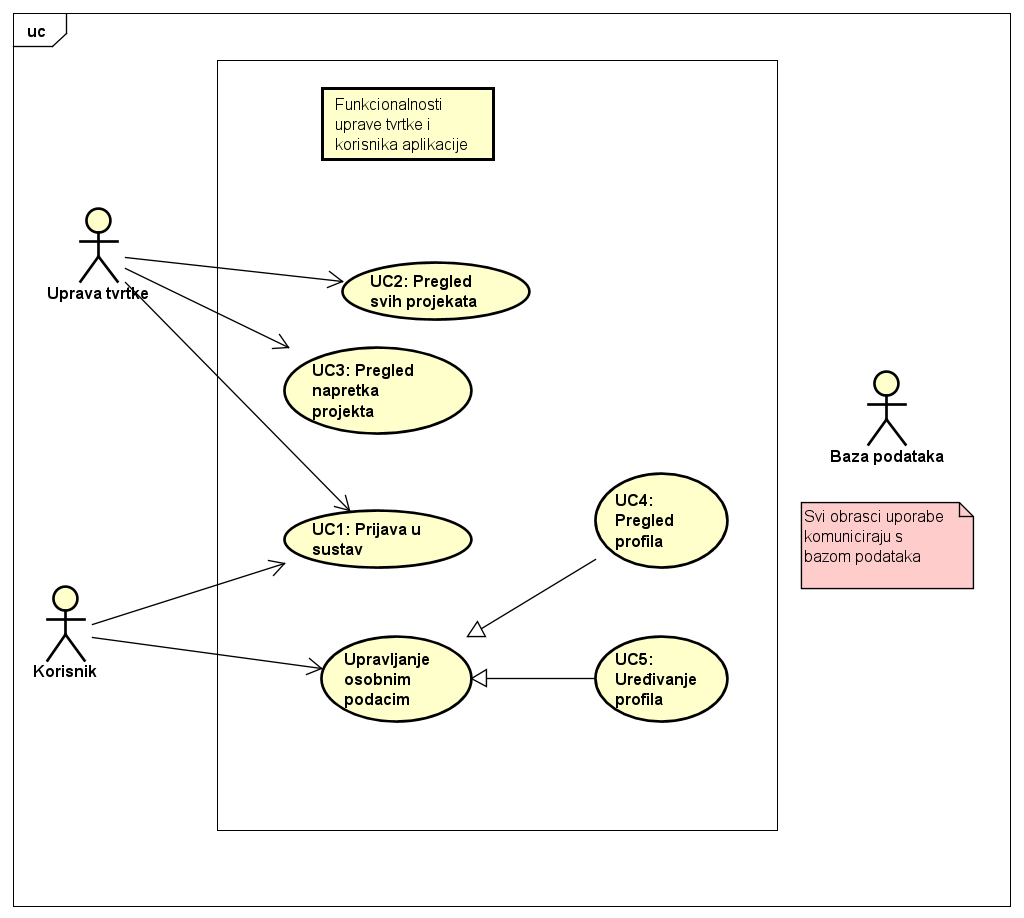
\includegraphics[width=\textwidth]{slike/funkc_korisnika_i_uprave.png}
						\caption{Dijagram obrasca uporabe, funkcionalnosti uprave tvrtke i korisnika}
					\end{figure}
					
					
					\begin{figure} 
						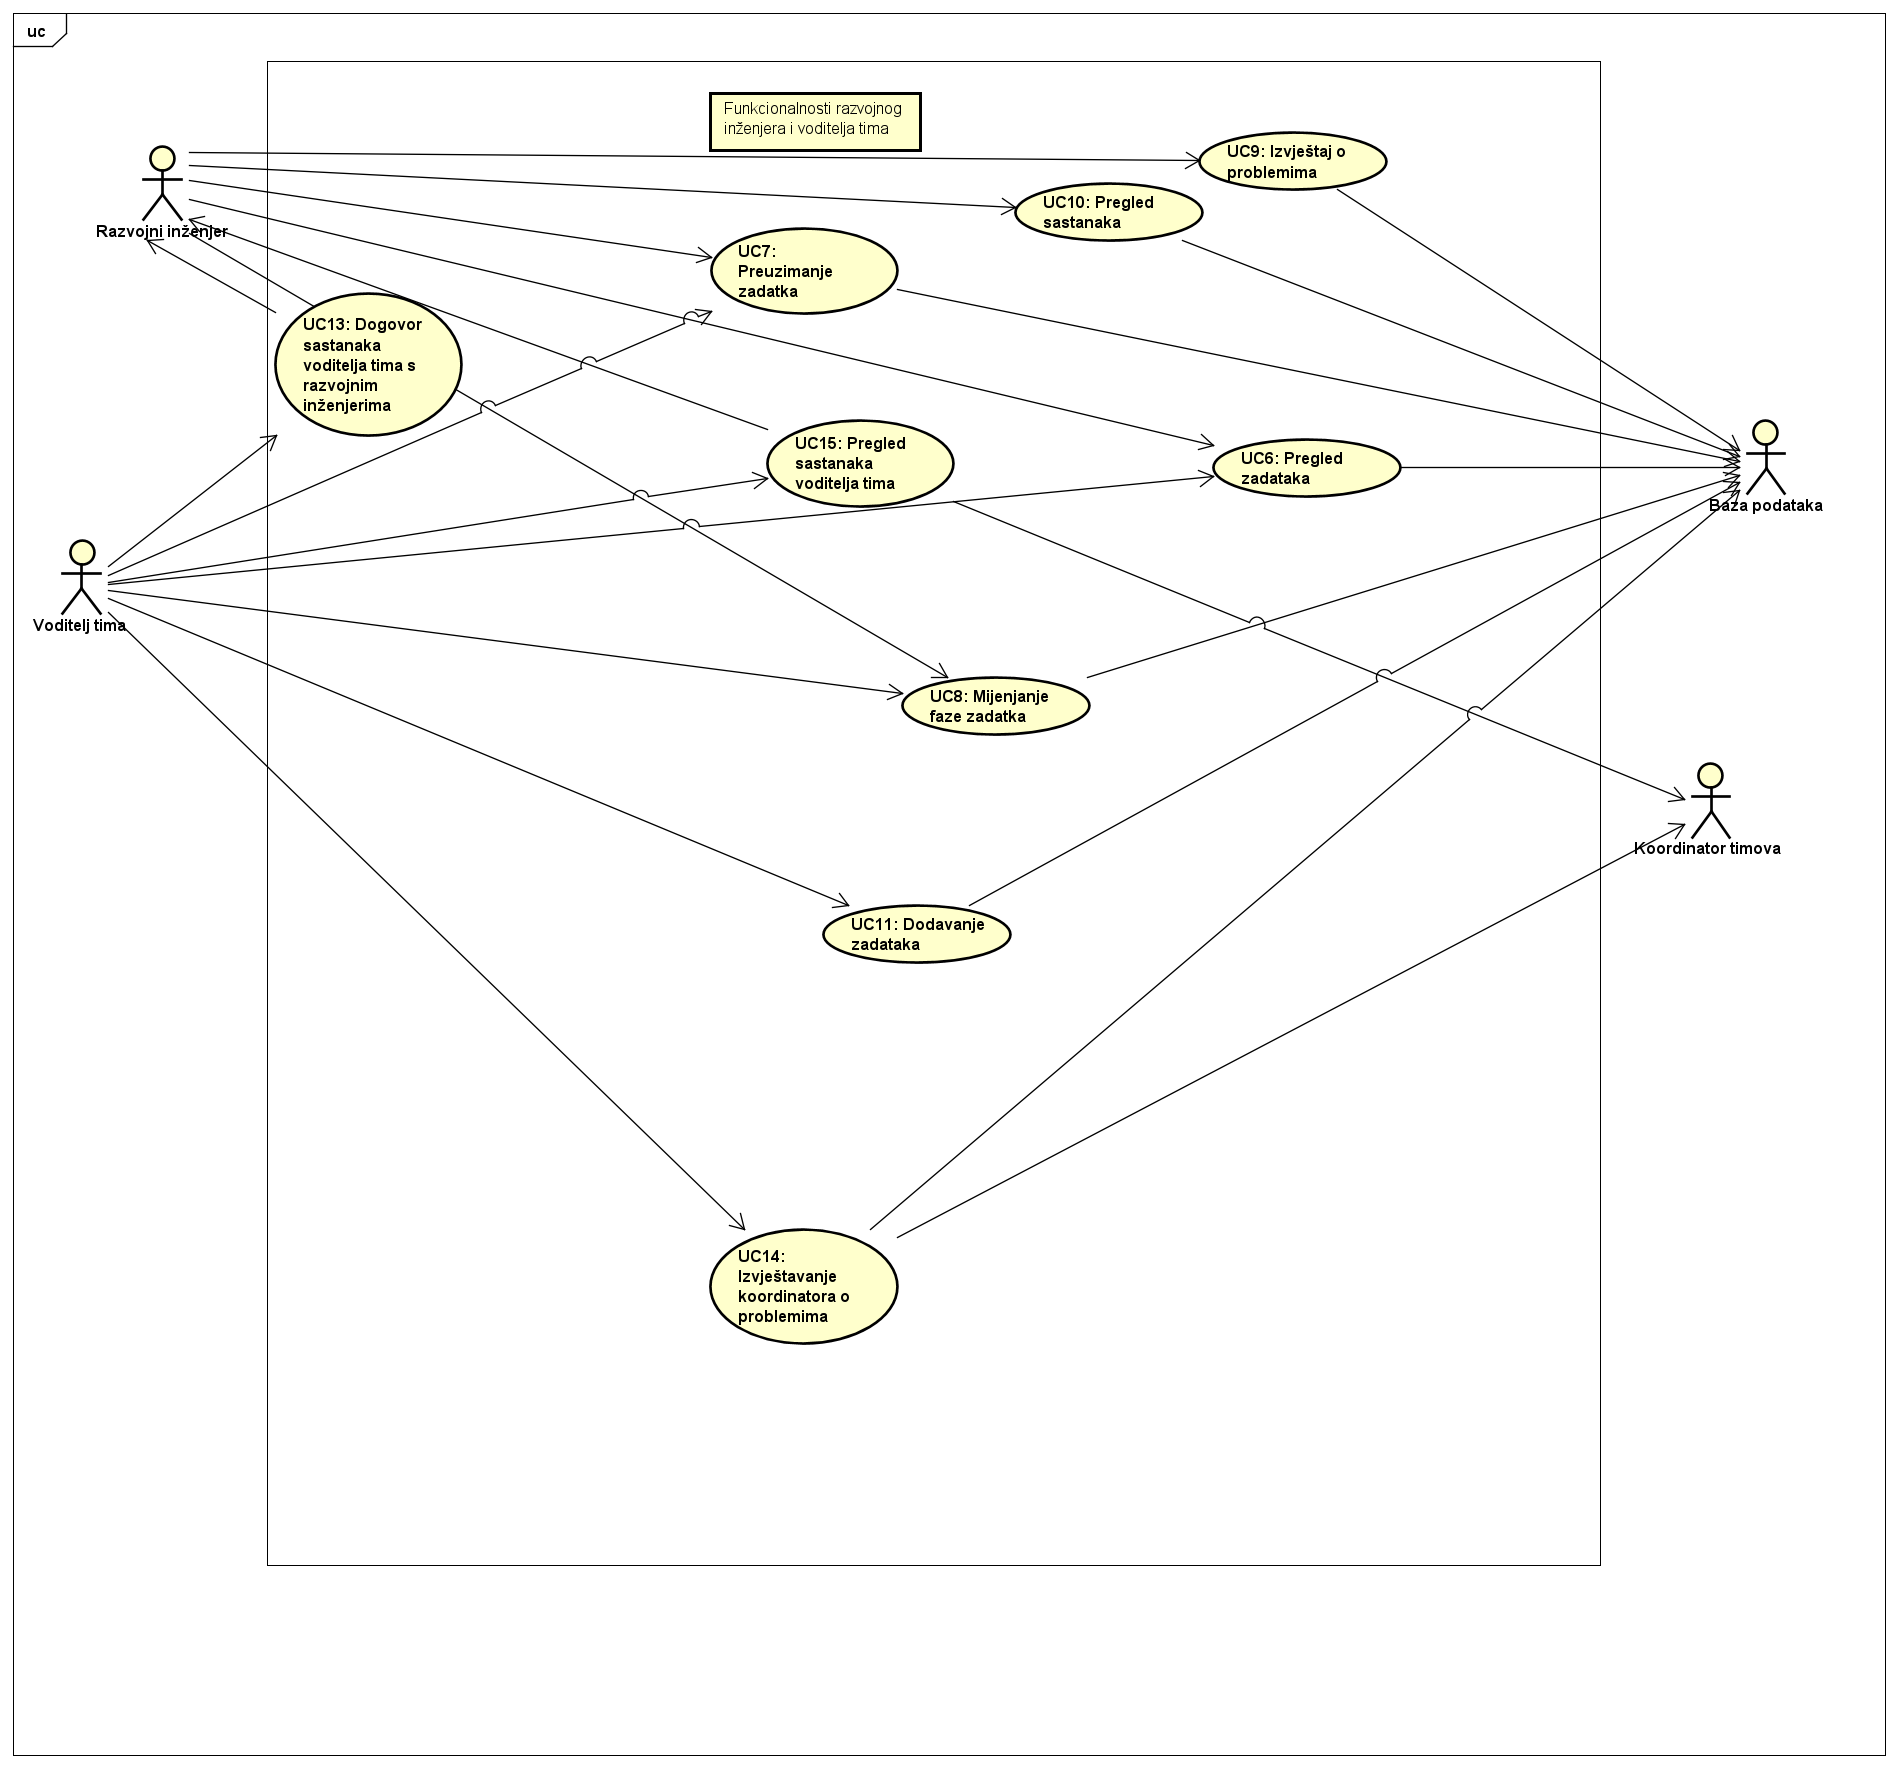
\includegraphics[width=\textwidth]{slike/funkc_razvojnog_inzenjera_i_voditelja.png}
						\caption{Dijagram obrasca uporabe, funkcionalnosti razvojnog inženjera i voditelja tima}
					\end{figure}
					
					\begin{figure} 
						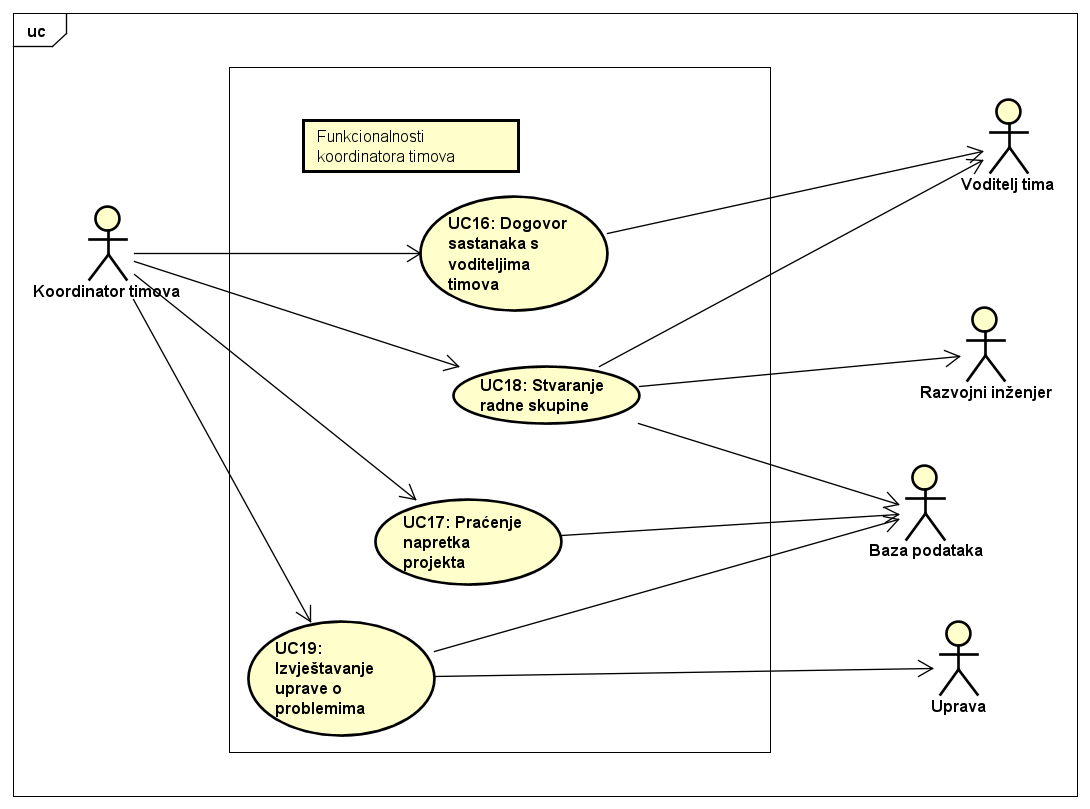
\includegraphics[width=\textwidth]{slike/funkc_koordinatora.png}
						\caption{Dijagram obrasca uporabe, funkcionalnosti koordinatora timova}
					\end{figure}
				\eject		
				
			\subsection{Sekvencijski dijagrami}
				
				\textbf{Obrazac uporabe UC1 - Prijava u sustav}

				\par Član uprave tvrtke unosi korisničko ime i lozinku kako bi se mogao prijaviti u sustav. Poslužitelj pomoću baze podataka provjerava postoji li uneseno korisničko ime i pripada li mu navedena lozinka. Ako su podaci točni članu uprave tvrtke odobrava se ulaz u sustav. Ukoliko podaci nisu ispravni, sustav obavještava člana uprave tvrtke o tome uz poruku. 
				\begin{figure}[h!]
				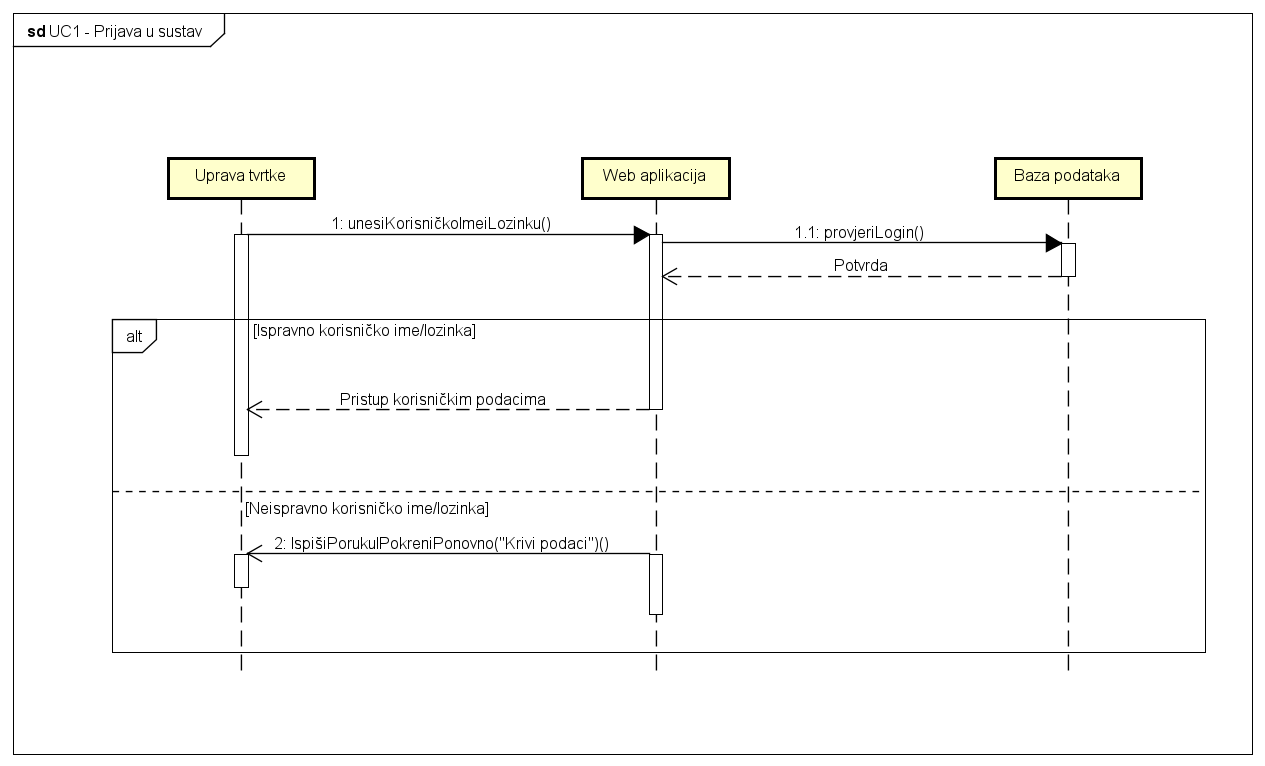
\includegraphics[width=\textwidth]{slike/Sekvencijski_UC1.png}
				\caption{Sekvencijski dijagram za UC1}
				\end{figure}
				\newpage
				\textbf{Obrazac uporabe UC5 - Uređivanje profila}
				
				\par Korisnik traži pristup svojem profilu kako bi ga mogao urediti. Poslužitelj dohvaća korisnikov profil i prikazuje ga. Korisnik na poslužitelju radi promjene prije nego odabere opciju spremanja promjena na profilu. Poslužitelj promjene profila prosljeđuje bazi podataka, a korisnik od poslužitelja traži izlazak iz uređivanja profila. Ukoliko korisnik nije spremio promijenjene podatke, a želi izaći iz uređivanja profila, poslužitelj ga obavještava o tome uz poruku.
				\begin{figure}[h!]
					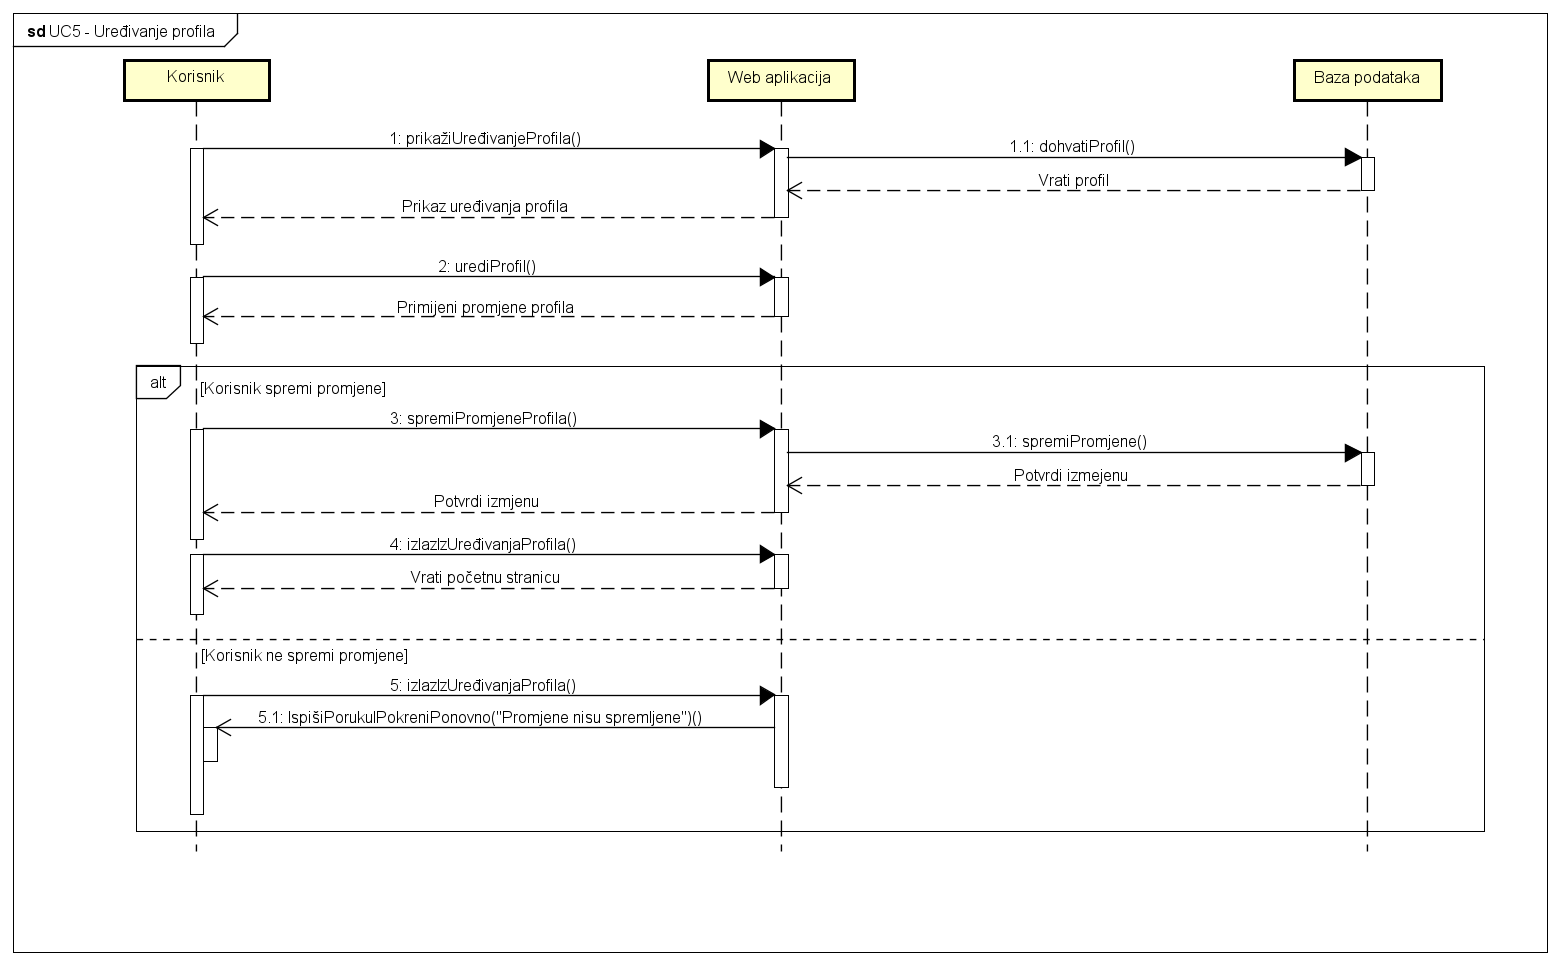
\includegraphics[width=\textwidth]{slike/Sekvencijski_UC5.png}
					\caption{Sekvencijski dijagram za UC5}
					\end{figure}
				\newpage
				\textbf{Obrazac uporabe UC11 - Dodavanje zadataka}
				
				\par Vođa tima odabire opciju za dodavanje novog zadatka. Poslužitelj korisniku vraća obrazac koji on treba popuniti za izradu novog zadatka. Vođa tima na poslužitelju popunjava obrazac za izradu novog zadatka. Vođa tima zatim potvrđuje i sprema novi zadatak. Ukoliko vođa tima nije upisao ime novog zadatka sustav ga obavještava o tome uz poruku. U suprotnom slučaju poslužitelj prosljeđuje novi zadatak u bazu podataka.
				\begin{figure}[h]
					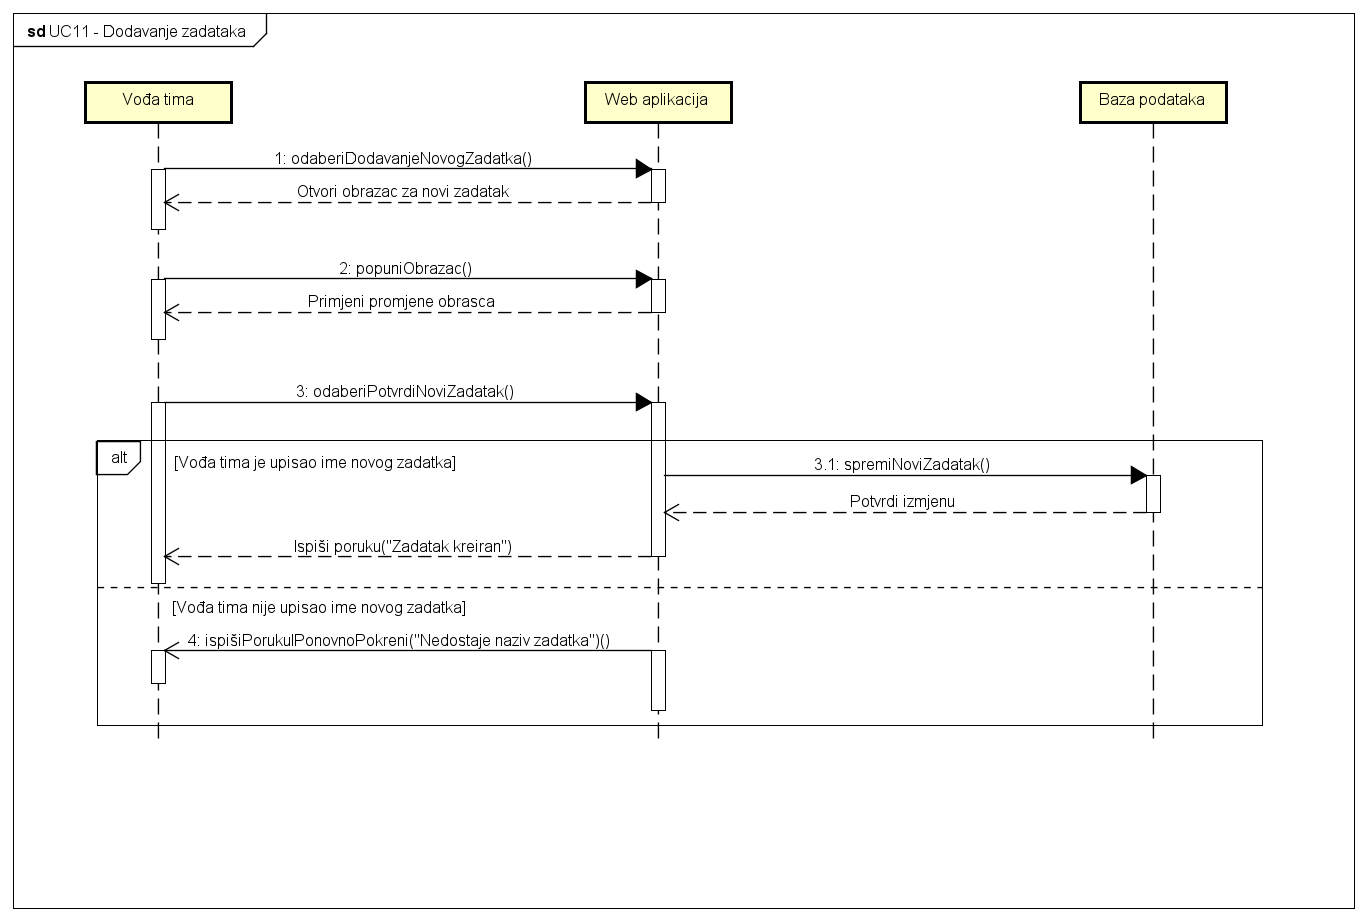
\includegraphics[width=\textwidth]{slike/Sekvencijski_UC11.png}
					\caption{Sekvencijski dijagram za UC11}
					\end{figure}
				\newpage
				\textbf{Obrazac uporabe UC18 - Stvaranje radne skupine}
				
				\par Koordinator traži prikaz radnih grupa. Poslužitelj dohvaća postojeće radne grupe i prikazuje ih. Koordinator  odabire opciju za izradu nove radne skupine zbog čega mu poslužitelj vraća obrazac za izradu nove radne skupine. Korisnik popuni obrazac nakon čega poslužitelj uspoređuje podatke iz obrasca s onima iz baze podataka. Ukoliko koordinator nije upisao ime radne skupine ili nije odabrao tim poslužitelj će ga obavijestiti uz pripadajuću poruku i nastaviti s ispunjavanjem obrasca. Ukoliko je kooordinator odabrao tim koji već pripada radnoj skupini ili je odabrao naziv koji se već koristi, također će biti obaviješten od strane poslužitelja i nastaviti će se s popunjavanjem obrasca. Kada su podaci ispravni koordinator želi napustiti obrazac. Ako je koordinator odabrao opciju spremanja radne skupine, onda ju poslužitelj sprema na bazu podataka. U suprotnom slučaju poslužitelj obaviještava koordinatora da nije spremio novu radnu skupinu.
				\begin{figure}[h]
					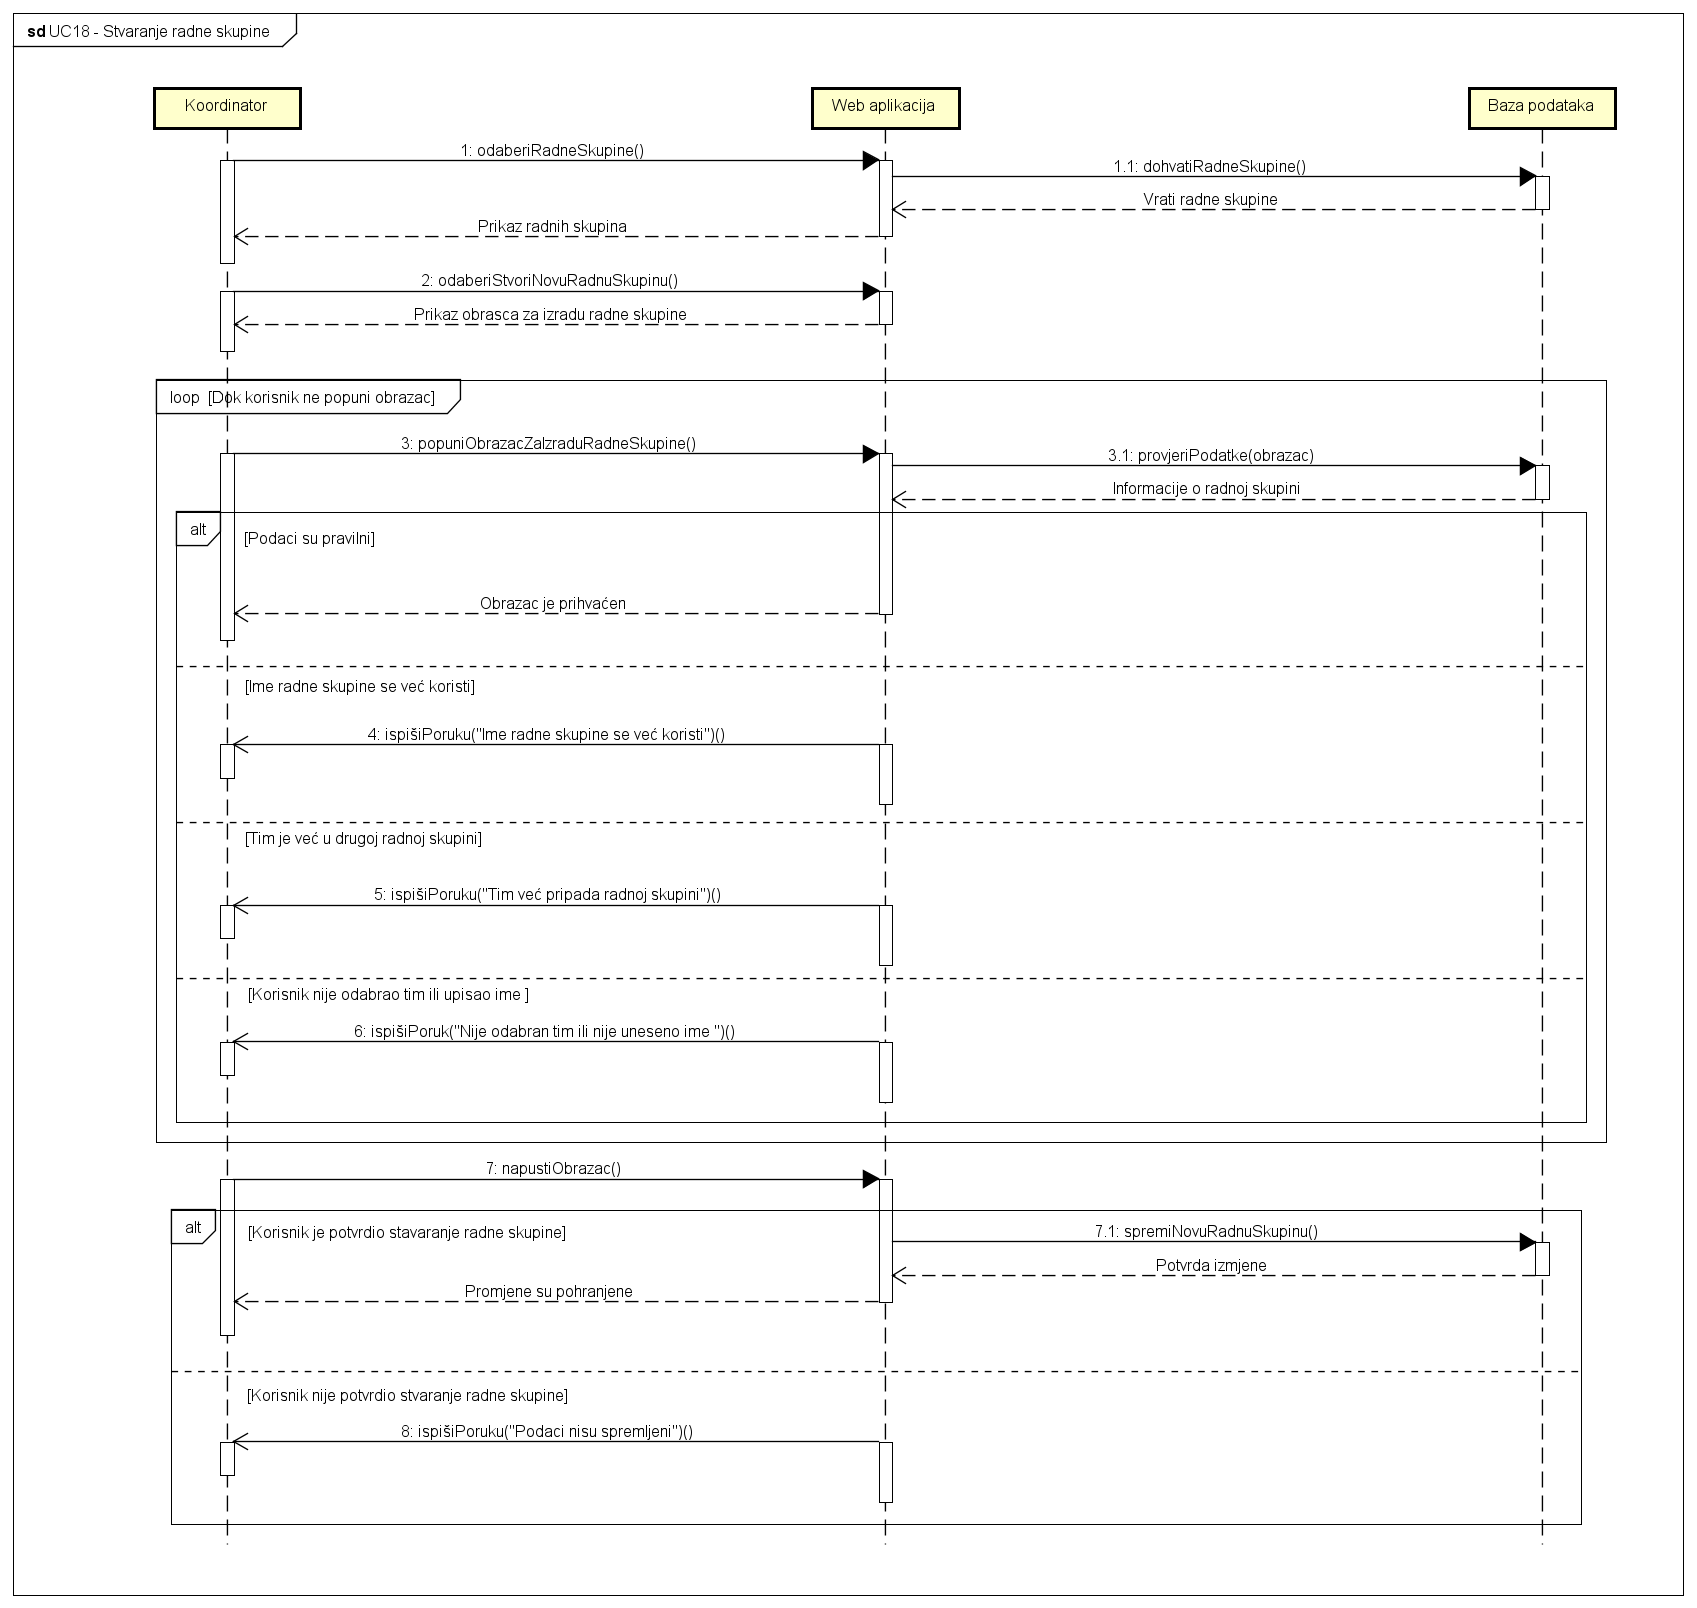
\includegraphics[width=\textwidth]{slike/Sekvencijski_UC18.png}
					\caption{Sekvencijski dijagram za UC18}
					\end{figure}
				\eject
				
		\pagebreak
		\newpage	
		\section{Ostali zahtjevi}
		
			 \begin{itemize}
			 \item Sustav mora podržavati rad za sve zaposlenike tvrtke istovremeno 
			 \item Korisničko sučelje i sustav moraju podržavati hrvatske znakove
			 \item Upiti bazi podataka moraju čekati najviše 3 sekunde
			 \item Sustav treba biti jednostavan i intuitivan za korištenje (KISS princip)
			 \item Sustav mora poštovati načelo nadogradnje uz minimalnu promjenu
			 \item Sustav za raspodjelu zadataka mora koristiti kanban ploču
			 \item za komunikaciju između klijenta i sustava mora biti korišten HTTPS protokol
			 \item veza s bazom podataka mora biti zaštićena, brza i otporna na vanjske greške
			 \item podaci se moraju sanirati prije slanja bazi podataka
			 \end{itemize}

	\chapter{Arhitektura i dizajn sustava}

	Arhitekturu web aplikacije dijelimo na tri podsustava:
	\begin{itemize}
	\item Web aplikacija
	\item Web poslužitelj
	\item Baza podataka
	\end{itemize}

	%slika arhitekture
	\begin{figure}[H]
		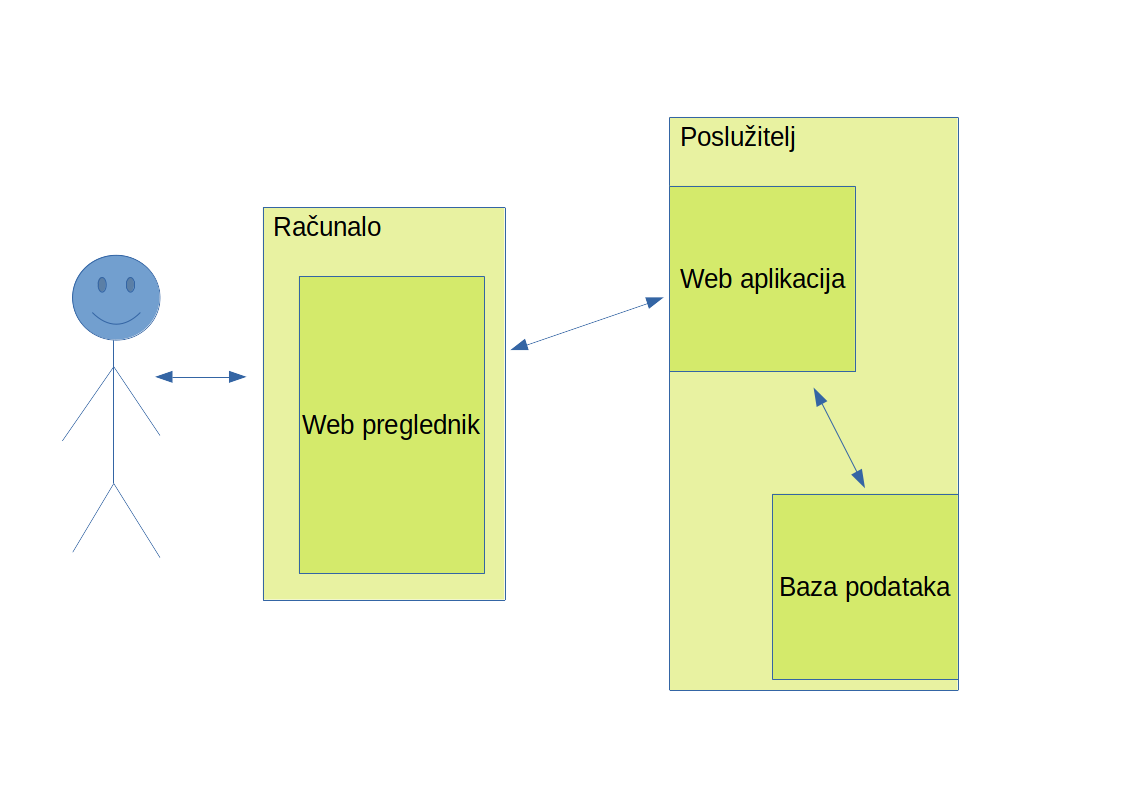
\includegraphics[width=\textwidth]{slike/arhitektura.png}
		\centering
		\caption{Arhitektura sustava}
		\label{fig:arhitektura_sustava}
	\end{figure}
	
	\underline{\textit{Web preglednik}} (eng. \textit{web browser}) je korisnički program koji omogućuje pregledavanje statičkih i dinamičkih sadržaja interneta. Web preglednik dohvaća sadržaj s lokalnog ili udaljenog računala, i potom taj sadržaj interpretira i prikazuje korisniku. Neki od popularnijih web preglednika današnjice su Chrome, Safari, Firefox i Edge.
	
	\underline{\textit{Web poslužitelj}} (eng. \textit{web server}) je temelj aplikacije, a služi za komunikaciju. Korisnik i aplikacija razmjenjuju HTTP zahtjeve (eng. \textit{HTTP request}) i HTTP odgovore (eng. \textit{HTTP response}). Poslužitelj pokreće prednji kraj (eng. \textit{front end}) i stražnji kraj (eng. \textit{back end}). Radi jednostavnosti, baza podataka je također smještena na poslužitelju.
	
	Korisnik kroz grafičko sučelje, odnosno prednji kraj, šalje zahtjeve na REST pristupne točke stražnjeg kraja. Tada stražnji kraj procesuira zahtjev i ako je potrebno komunicira s bazom podataka. Nakon konstrukcije, stražnji kraj šalje odgovor prednjem kraju u obliku JSON objekta, a prednji kraj procesuira odgovor i promjene prikazuje korisniku u obliku HTML stranice. 
	
	Za aplikaciju je odabrana višeslojna arhitektura temeljena na \textbf{MVC} (\textit{model-view-controller}) arhitekturnom stilu te uslužnoj arhitekturi. Podjelu slojeva možemo napraviti na idući način:
	\begin{figure}[H]
		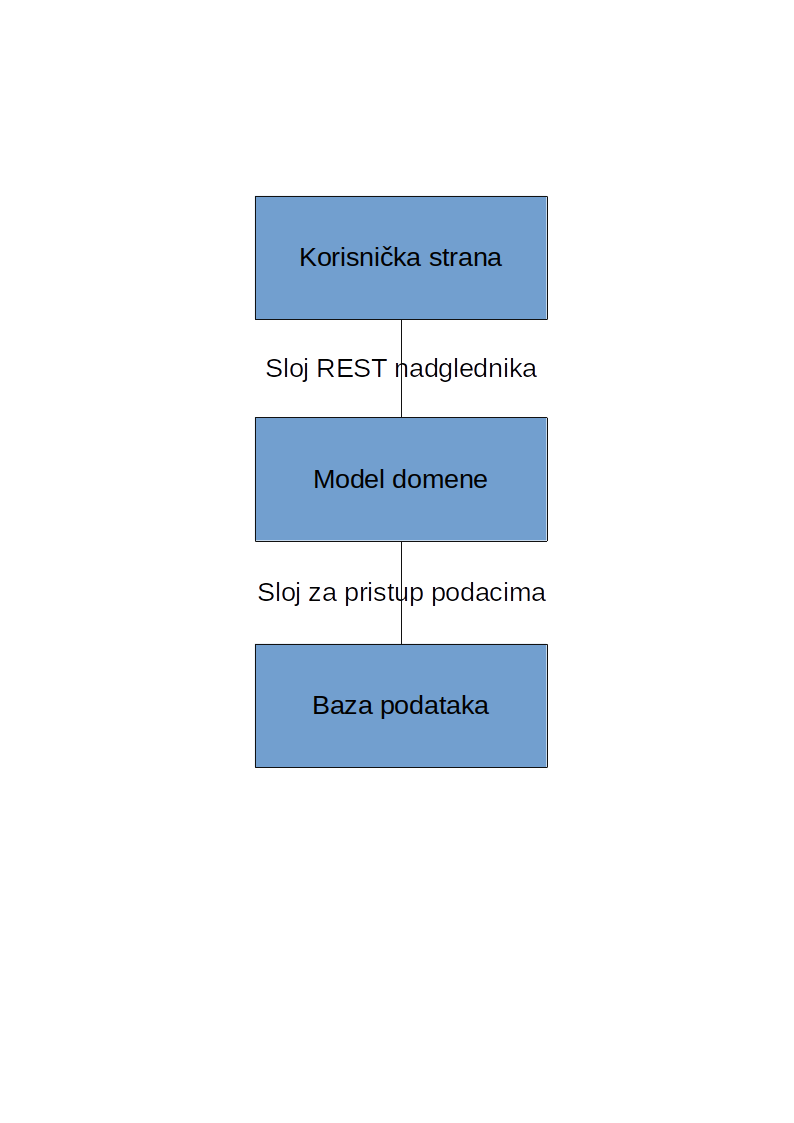
\includegraphics[scale=0.3]{slike/slojevita_arhitektura.png}
		\centering
		\caption{Podjela slojeva}
		\label{fig:podjela_slojeva}
	\end{figure}
	\begin{enumerate}
		\item \textit{sloj korisničke strane} - korisničko sučelje implementirano u JavaScriptu i radnom okviru AngularJS
		\item \textit{sloj nadglednika} - REST nadglednici 
		\item \textit{sloj domene} - model podataka iz domene primjene
		\item \textit{sloj za pristup podacima} - posrednik između sloja domene i baze podataka
		\item \textit{sloj baze podataka} - pohrana podataka
	\end{enumerate}
	
	Ovakva arhitektura odabrana je zbog poželjnih svojstava MVC arhitekturnog stila i višeslojne arhitekture: razvoj pojedinih slojeva jednostavniji je i u velikom stupnju nezavisan od razvoja drugih slojeva. Također, komunikacija prednjeg i stražnjeg kraja je ostvarena primjenom REST arhitketurnog stila. Zbog toga su prednji i stražnji kraj neovisni u smislu jezika implementacije, što potiće ponovnu uporabu.
	
	MVC arhitekturni stil sastoji se od tri koncepta:
	\begin{itemize}
		\item \textbf{Model} - reprezentacija strukture podataka koja se koristi u rješenju, neovisna o korisničkom sučeju
		\item \textbf{View} - pogled na podatke, u našoj aplikaciji to je grafičko sučelje
		\item \textbf{Controller} - nadzornik koji koordinira zahtjeve i odgovore između modela i pogleda, sadrži svu logiku upravljanja.
	\end{itemize}

	REST (\textit{representational state transfer}) arhitekturni stil kao upite koristi URI-je koji su mu poslani i tip HTTP zahtjeva, a odgovara JSON objektom. Tip HTTP zahtjeva koristi se za dohvat, ažuriranje ili umetanje podataka u bazu podataka, a dijelovi URI-ja se koriste za specificiranje zahtjeva. Tako bi na primjer REST API na GET upit usmjeren na putanju /employees odgovorio nizom koji sadrži sve zaposlenike, a GET upit na putanju /employees/user27 bi dobio odgovor JSON objekt koji predstavlja zaposlenika s korisničkim imenom user27.
	
		

				
		\section{Baza podataka}
			
		Odabrali smo PostgreSQL relacijsku bazu podataka za našu web aplikaciju zbog široke korisničke podrške, dokazane stabilnosti, dostupnosti sučelja s Javom, te prijašnjeg iskustva u radu s njom. Relacijska baza podataka omogućuje jednostavno modeliranje problema domene, a temeljna joj je zadaća sigurna i brza pohrana i dohvaćanje podataka. Temeljna građevna jedinica baze podataka je relacija (tablica). Jedna relacija predstavlja jedan entitet, a naša baza sastoji se od idućih relacija:
			
		\begin{itemize}
			\item employees
			\item projects
			\item tasks
			\item teams
			\item workgroups
		\end{itemize}
		
			\subsection{Opis tablica}
			
				\textbf{employees} - Ovaj entitet predstavlja zaposlenika. Sadrži atribute ID, korisničko ime, ime, prezime, lozinka, email, broj telefona, funkciju u firmi te ID tima kojemu pripada. U vezi je \textit{One-to-Many} s entitetom tasks preko atributa ID i u vezi \textit{Many-to-One} s entitetom teams preko atributa ID.		
				\begin{longtabu} to \textwidth {|X[6, l]|X[6, l]|X[20, l]|}
					
					\hline \multicolumn{3}{|c|}{\textbf{employees}}	 \\[3pt] \hline
					\endfirsthead
					
					\hline 
					\endlastfoot
					
					\textbf{emp\_id} & BIGINT	&  jedinstveni identifikator zaposlenika\\ \hline
					emp\_name & VARCHAR & ime zaposlenika \\ \hline
					emp\_surname & VARCHAR & prezime zaposlenika \\ \hline
					emp\_username & VARCHAR & zaposlenikovo korisničko ime \\ \hline
					emp\_password & VARCHAR & zaposlenikova lozinka \\ \hline
					emp\_email & VARCHAR & zaposlenikov email \\ \hline
					emp\_phone & VARCHAR & zaposlenikov broj telefona \\ \hline
					emp\_clearance & INT & zaposlenikova funkcija - developer, team lead, koordinator ili uprava \\ \hline
					\textit{team\_id}	& BIGINT & identifikacijski broj tima kojemu zaposlenik pripada, (teams.team\_id)\\ \hline 		
				\end{longtabu}
			
			
				\textbf{projects} - Ovaj entitet predstavlja projekt. Sadrži atribute ID, opis, ime, te ID tima koji ga je preuzeo. U vezi je \textit{One-to-One} s entitetom teams preko atributa ID tima koji ga je preuzeo.
				\begin{longtabu} to \textwidth {|X[6, l]|X[6, l]|X[20, l]|}
					
					\hline \multicolumn{3}{|c|}{\textbf{projects}}	 \\[3pt] \hline
					\endfirsthead
					
					\hline 
					\endlastfoot
					
					\textbf{project\_id} & BIGINT	&  jedinstveni identifikator projekta\\ \hline
					project\_desc	& VARCHAR & opis projekta	\\ \hline 
					project\_name & VARCHAR &  ime projekta \\ \hline 
					\textit{team\_team\_id} & BIGINT	&  identifikator tima koji rješava projekt, (teams.team\_id)	\\ \hline 					
				\end{longtabu}
			
				\textbf{tasks} - Ovaj entitet predstavlja zadatak na kanban ploči. Sadrži atribute ID, ime, opis, prioritet, status, ID zaposlenika koji ga je preuzeo, te ID tima kojemu pripada. U vezi je \textit{Many-to-One} s entitetom teams preko atributa ID tima kojemu pripada. U istoj je vezi s entitetom employees preko atributa ID korisnika koji ga je preuzeo.
				\begin{longtabu} to \textwidth {|X[6, l]|X[6, l]|X[20, l]|}
					
					\hline \multicolumn{3}{|c|}{\textbf{tasks}}	 \\[3pt] \hline
					\endfirsthead					
					\hline 
					\endlastfoot
					
					\textbf{task\_id} & INT	& jedinstveni identifikator zadatka	\\ \hline
					task\_deadline	& TIMESTAMP &  rok predaje zadatka 	\\ \hline 
					task\_desc & VARCHAR & opis zadatka \\ \hline 
					task\_name & VARCHAR	& ime zadatka\\ \hline 
					task\_prio & INT & prioritet zadatka \\ \hline
					task\_status & INT & status napretka zadatka\\ \hline 
					\textit{emp\_id}	& BIGINT & identifikator zaposlenika koji rješava zadatak, (employee.emp\_id) \\ \hline 
					\textit{team\_id} & BIGINT & identifikator tima kojemu ovaj zadatak pripada, (teams.team\_id)\\ \hline
					
					
				\end{longtabu}
			
			
				\textbf{teams} - Ovaj entitet predstavlja tim zaposlenika u firmi. Sadrži atribute ID tima te ID radne skupine kojoj tim pripada. U vezi je \textit{Many-to-One} s entitetom workgroups preko atributa ID radne skupine kojoj tim pripada i u vezi \textit{One-to-Many} s entitetom employees preko atributa ID. U istoj vezi je s entitetom tasks preko atributa ID. Također je u vezi \textit{One-to-Many} s entitetom projects preko atributa ID.
				\begin{longtabu} to \textwidth {|X[6, l]|X[6, l]|X[20, l]|}
					
					\hline \multicolumn{3}{|c|}{\textbf{teams}}	 \\[3pt] \hline
					\endfirsthead					
					\hline 
					\endlastfoot
					
					\textbf{team\_id} & BIGINT & jedinstveni identifikator tima	\\ \hline
					\textit{wg\_id}	& BIGINT & identifikator radne skupine kojoj ovaj tim pripada, (workgroups.wg\_id)	\\ \hline 
				\end{longtabu}
			
				\textbf{workgroups} - Ovaj entitet predstavlja radnu skupinu. Radna skupina sastoji se od više timova i ima jednog koordinatora. Sadrži atribute ID radne skupine, te ID koordinatora tima. U vezi je \textit{One-to-One} s entitetom employees preko atributa ID koordinatora tima, te je u vezi \textit{One-To-Many} s entitetom teams preko atributa ID radne skupine.
				\begin{longtabu} to \textwidth {|X[10, l]|X[6, l]|X[20, l]|}
					
					\hline \multicolumn{3}{|c|}{\textbf{workgroups}}	 \\[3pt] \hline
					\endfirsthead
					\hline 
					\endlastfoot
					
					\textbf{wg\_id}		 & BIGINT	&  jedinstveni identifikator radne skupine 	\\ \hline
					\textit{coordinator\_emp\_id} 	& BIGINT & identifikator zaposlenika koji je koordinator ove radne skupine  	\\ \hline 
				\end{longtabu}
			
			
			\subsection{Dijagram baze podataka}
			\begin{figure}[H]
				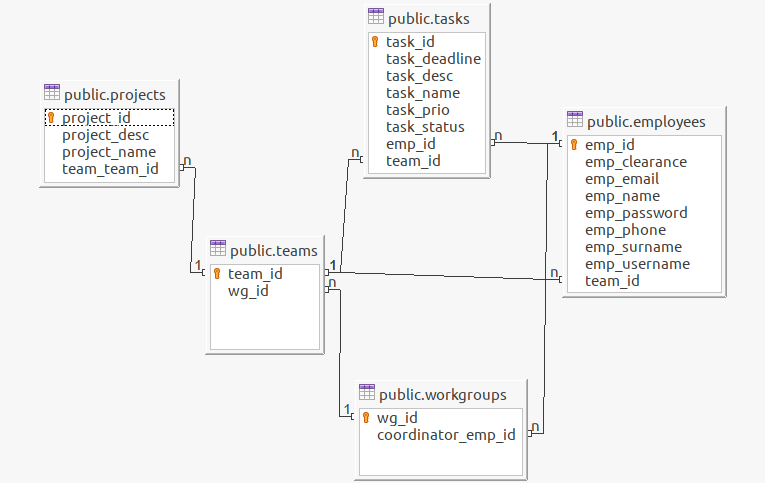
\includegraphics[width=\textwidth]{slike/dijagram_baze.png}
				\centering
				\caption{Dijagram baze podataka}
				\label{fig:dijagram_baze}
			\end{figure}
			
			\eject
			
			
		\section{Dijagram razreda}
		
			Dijagram razreda prikazuje odnose između različitih objekata, te njihove atribute i operacije kojima vladaju. Na slikama 4.3, 4.4 i 4.5 prikazani su razredi koji pripadaju \textit{backend} dijelu naše arhitekture. Radi jednostavnosti, dijagram razreda je podijeljen u više slika, no bez obzira na to, prikazani razredi na neki način komuniciraju.
 			
 			
 			
 			Na idućoj slici prikazan je model podataka kojima backend rukuje. Zaposlenik u firmi modeliran je razredom Employee. Razred Team modelira tim zaposlenika u firmi. Razred Task modelira jedan zadatak na kanban ploči. Razred WorkGroup modelira radnu skupinu u firmi. Razred Project modelira projekt na kojem tim radi.
 			
			\begin{figure}[H]
				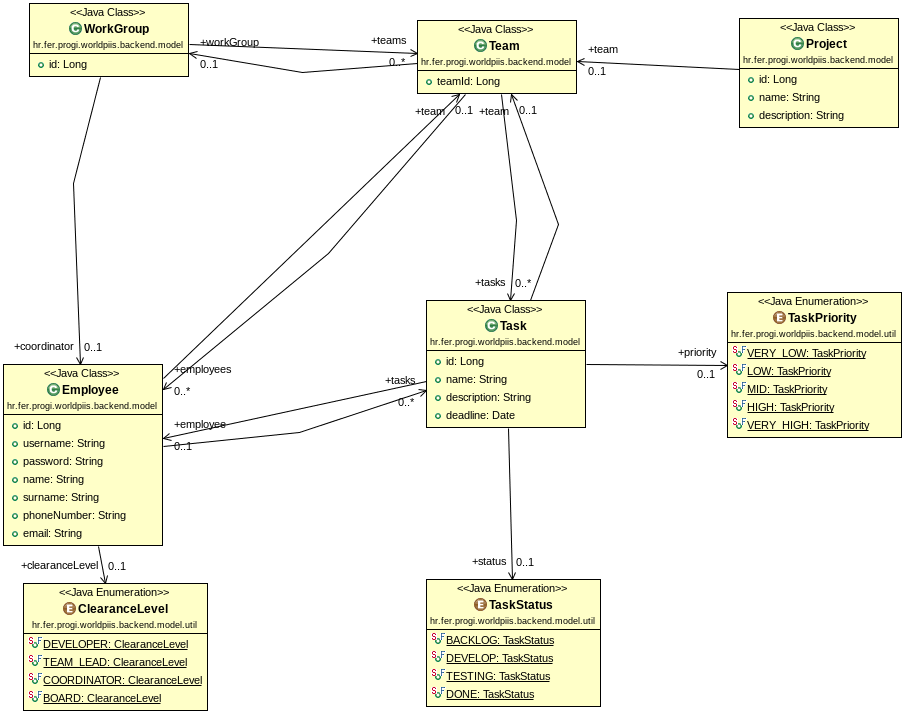
\includegraphics[width=\textwidth]{slike/CLASSD_model.png}
				\centering
				\caption{Dijagram razreda koji opisuje model}
				\label{fig:classd_model}
			\end{figure}
			
			Na idućoj slici prikazana je sredina backenda. Glavni objekt ovdje je sučelje CrudRepository, koje predstavlja apstraktni repozitorij podataka. Iz tog sučelja, izvedena su sučelja ProjectRepository, TaskRepository, TeamRepository, WorkGroupRepository i EmployeeRepository. Ta sučelja predstavljaju repozitorij podataka za prije navedene razrede modela, tj. oni predstavljaju poveznicu s bazom, ili DAO (eng. \textit{Data Access Object}).  
			\begin{figure}[H]
				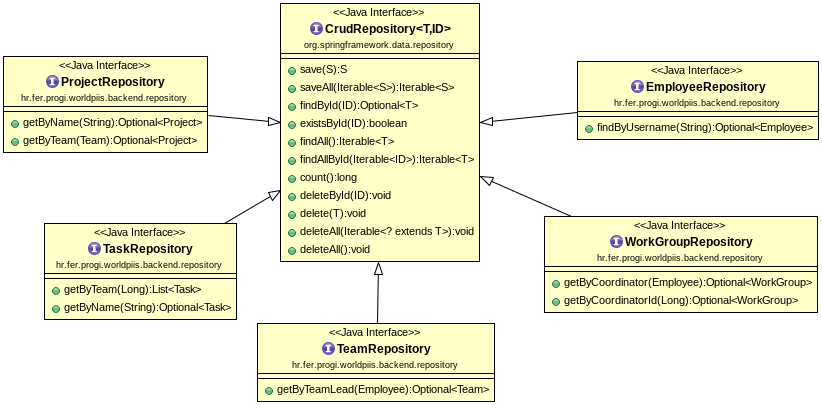
\includegraphics[width=\textwidth]{slike/CLASSD_middle.png}
				\centering
				\caption{Dijagram razreda koji opisuje sredinu backenda}
				\label{fig:classd_middle}
			\end{figure}
		
			Na idućoj slici prikazan je "frontend backenda", odnosno sučelje backenda prema stvarnome svijetu. Ovdje vidimo razrede EmployeeController, TeamController, TaskController, ProjectController i WorkGroupController. Svi ti razredi implementiraju sučelje RestController koje predstavlja REST endpoint. Ti razredi su oni koji dobivaju zahtjeve iz vanjskog svijeta, a odgovaraju HTTP odgovorima i JSON objektima. 
			\begin{figure}[H]
			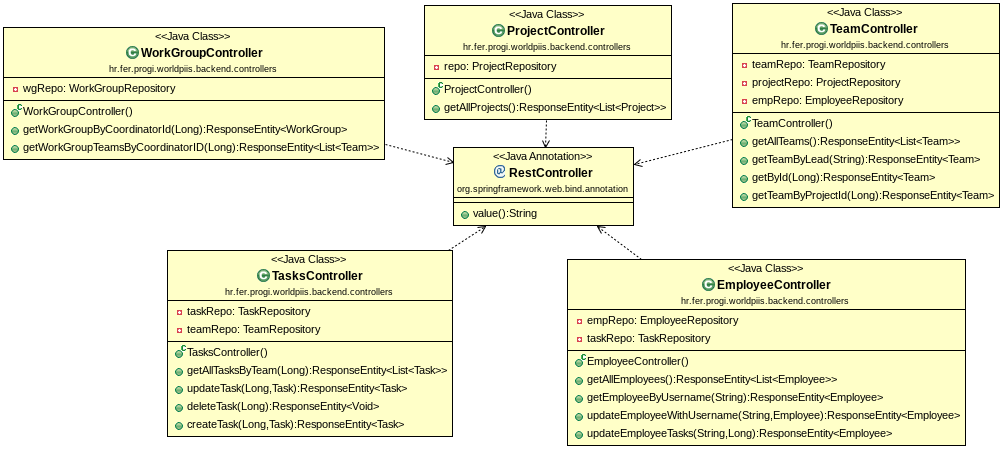
\includegraphics[width=\textwidth]{slike/CLASSD_controllers.png}
			\centering
			\caption{Dijagram razreda koji opisuje prednji dio backenda tj. kontrolere}
			\label{fig:classd_controllers}
			\end{figure}
			\eject
		
		\section{Dijagram stanja}
			
			Dijagram stanja primjenjuje se za opis stanja objekta i za opisivanje prijelaza iz jednog u drugo stanje. Priložena slika prikazuje dijagram stanja objekta "Zadatak". Vođa tima kreira novi zadatak te nakon toga on prelazi u stanje "Backlog". Zadatak u tom stanju preuzima neki razvojni inžinjer ili vođa tima zatim se vraća u to isto stanje. Zaposlenik može započeti razvoj ili testiranje zadataka koji time prelazi u odgovarajuće stanje. Zadatak može ući u stanje "Uređivanje" iz bilo kojeg drugog stanja. U završno stanje dolazi se nakon stanja "Done" što znači da je zadatak izvršen.
			\begin{figure}[H]
				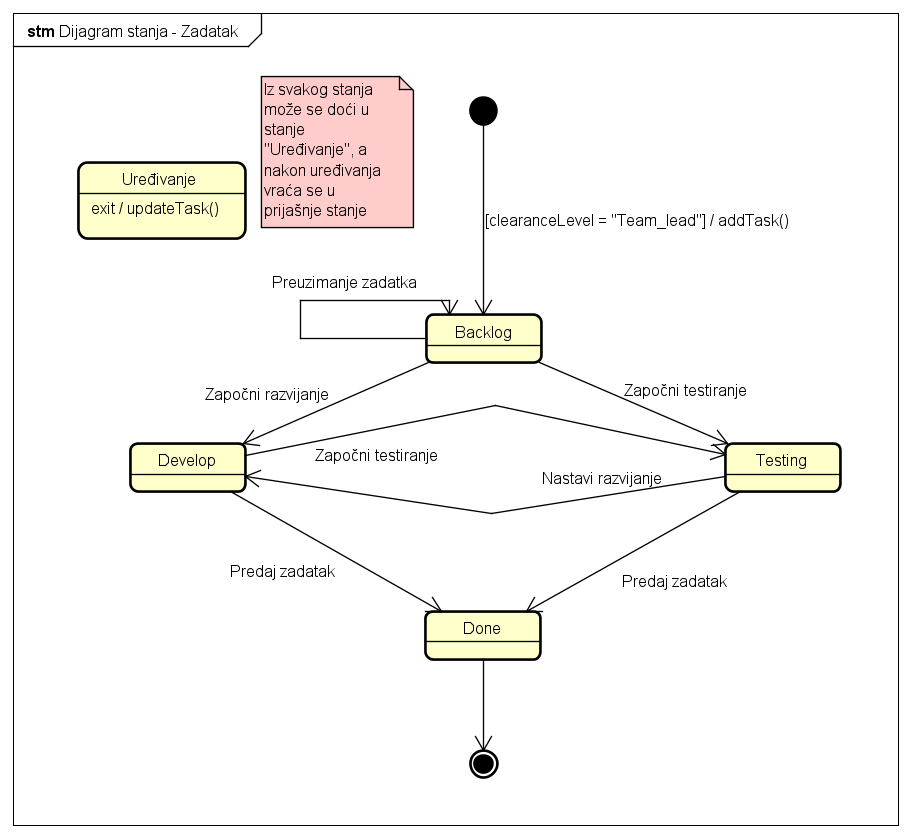
\includegraphics[width=\textwidth]{slike/Dijagram_stanja.png}
				\centering
				\caption{Dijagram stanja}
				\label{fig:classd_middle}
			\end{figure}
			
			
			\eject 
		
		\section{Dijagram aktivnosti}
			
			Dijagram aktivnosti prikazuje povezane aktivnosti na visokoj apstrakcijskoj razini. Dijagram aktivnosti intuitivno prikazuje kako podaci teku kroz aplikaciju i kako se kontrola nad podacima mijenja. Idući dijagram prikazuje proces preuzimanja zadatka i mijenjanja opisa zadatka. Ovaj proces može provesti neki razvojni inženjer ili voditelj tima.
			\begin{figure}[H]
				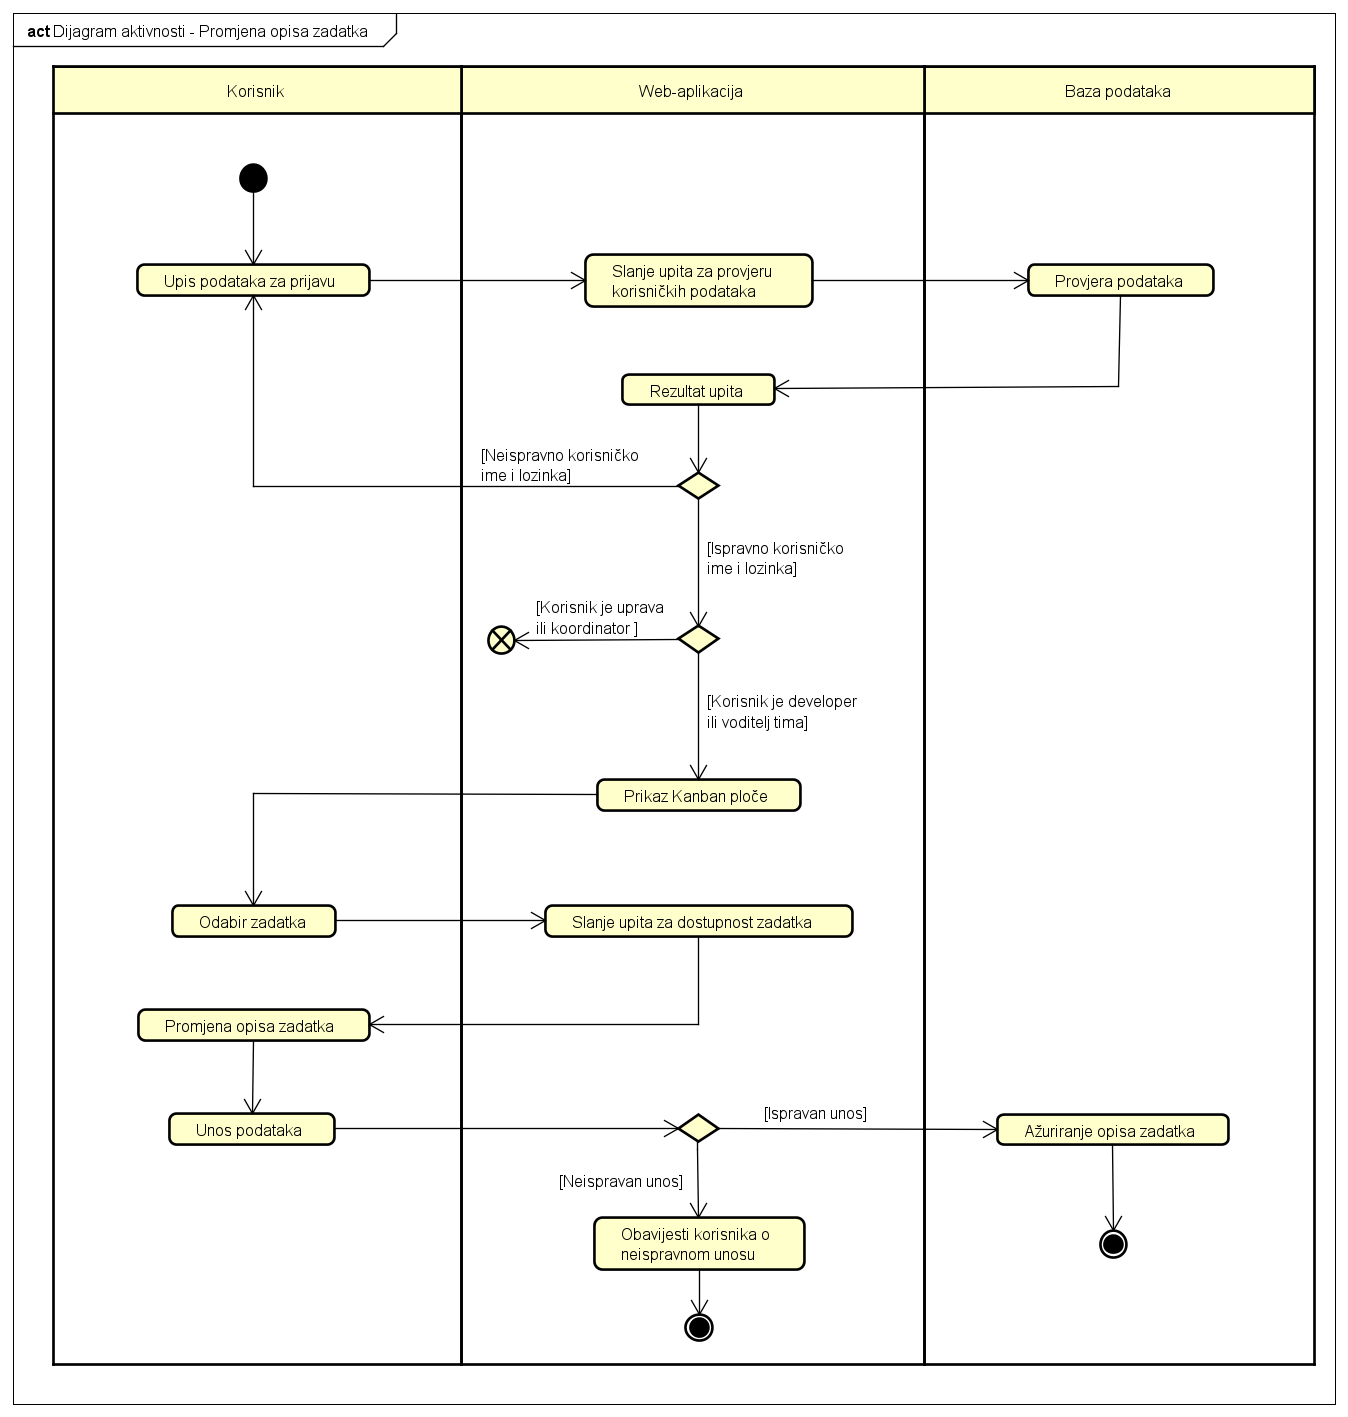
\includegraphics[width=\textwidth]{slike/dijagram_aktivnosti.png}
				\centering
				\caption{Dijagram aktivnosti}
				\label{fig:classd_middle}
			\end{figure}
			
			\eject
		
		\section{Dijagram komponenti}
		
		    Dijagram komponenti omogućuje nam pogled na sustav s visoke razine apstrakcije. Web aplikacija komunicira sa sustavom preko dva sučelja. Prvo sučelje služi za dohvat samih stranica, dakle HTML, CSS i JS datoteka. Drugo sučelje služi za komunikaciju između aplikacije i baze podataka. Dakle, web aplikacija šalje zahtjev REST API-u, koji zauzvrat preko kontrolera komunicira s repozitorijima podataka, koji predstavljaju sloj povezanosti između baze podataka i kontrolera. Repozitoriji dohvaćaju podatke iz baze, preoblikuju ih na način kako je to zapisano u modelima, i prosljeđuju ih kontrolerima. Ovakav način obrade podataka karakterističan je za MVC obrazac. 	
            \begin{figure}[H]
				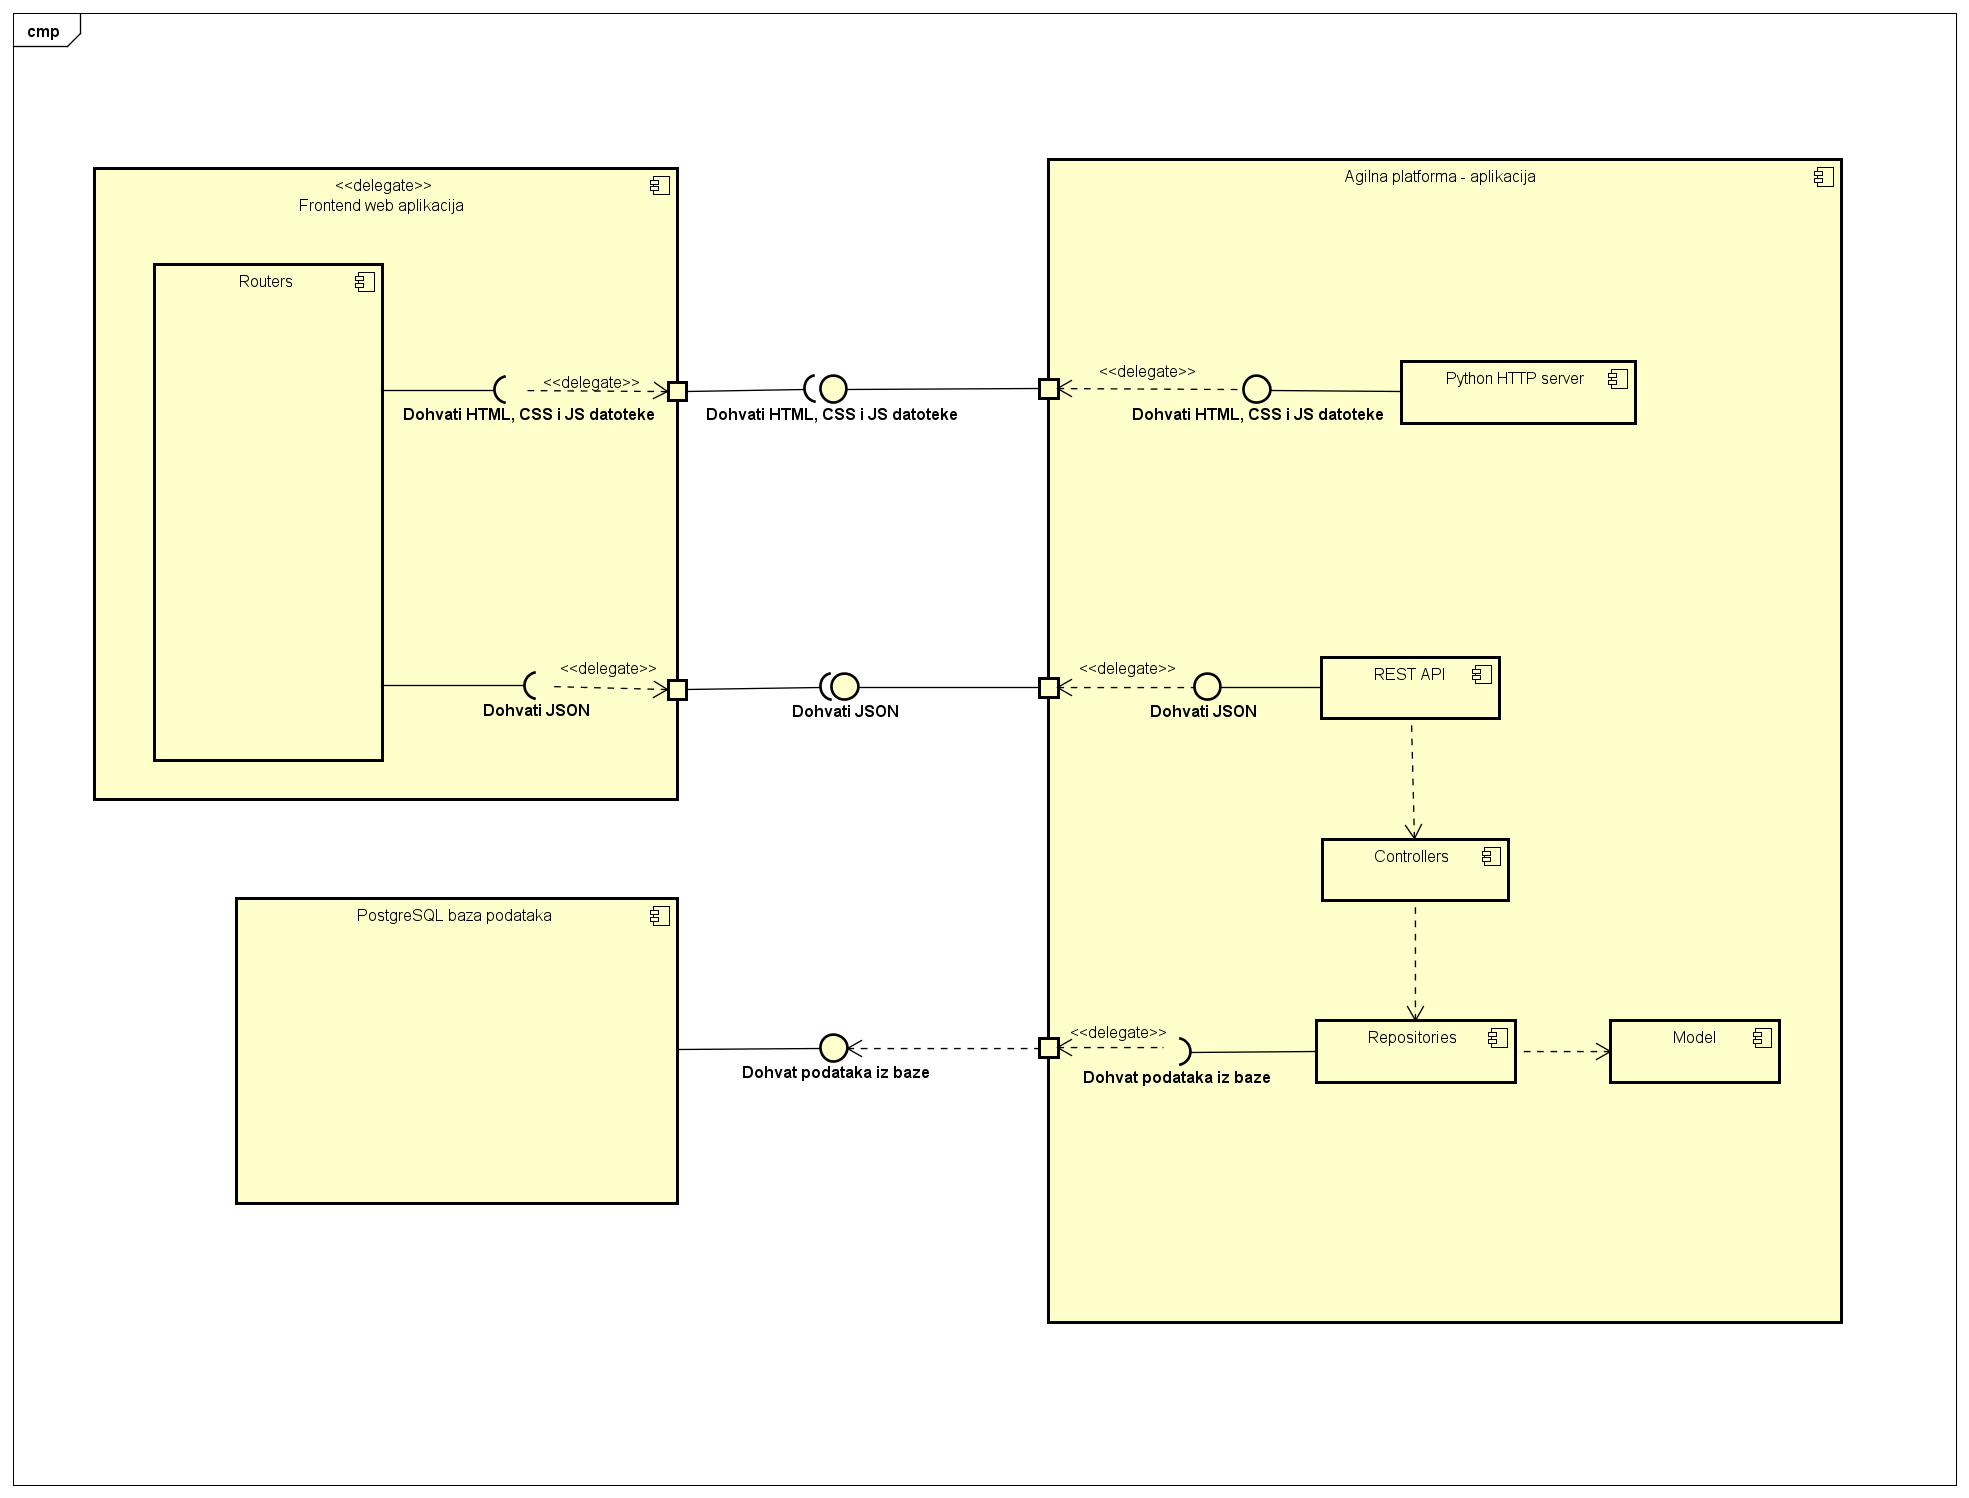
\includegraphics[width=\textwidth]{slike/dijagram_komponenti.png}
				\centering
				\caption{Dijagram komponenti}
				\label{fig:classd_middle}
			\end{figure}

	\chapter{Implementacija i korisničko sučelje}
		
		
		\section{Korištene tehnologije i alati}
		
			
			Komunikacija u timu realizirana je korištenjem platforme \underline{Microsoft Teams}\footnote{\url{https://www.microsoft.com/hr-hr/microsoft-365/microsoft-teams/}}. 
			Za izradu UML dijagrama korišten je alat \underline{Astah Professional}\footnote{\url{https://astah.net/products/astah-professional/}}, a kao sustav za upravljanje izvornim kodom \underline{Git}\footnote{\url{https://git-scm.com/}}. 
			Udaljeni repozitorij projekta je dostupan na web platformi \underline{GitLab}\footnote{\url{https://gitlab.com/}}.
			\par
			Kao razvojno okruženje korišten je \underline{IntelliJ IDEA}\footnote{\url{https://www.jetbrains.com/idea/}} - integrirano razvojno okruženje (IDE) tvrtke JetBrains. 
			Prvenstveno se koristi za razvoj računalnih programa za operacijski sustav Windows, kao i za web-stranice, web-aplikacije, web-usluge i mobilne aplikacije.
			\par
			Za razvoj korisničkog sučelja i frontenda korišten je uređivač teksta \underline{VSCode}\footnote{\url{https://code.visualstudio.com/}}. Taj uređivač teksta je danas jedan od najrasprostranjenijih i koristi se u svim sferama industrije. 
            \par
            Aplikacija je napisana u \underline{Javi}\footnote{\url{https://www.java.com/en/}} koristeći ekosustav \underline{Java Spring}\footnote{\url{https://spring.io/}} za
            izradu backenda te \underline{AngularJS}\footnote{\url{https://angularjs.org/}} i jezik \underline{JavaScript}\footnote{\url{https://www.javascript.com/}} za izradu frontenda. 
            \par
            Baza podataka (\underline{PostgreSQL}\footnote{\url{https://www.postgresql.org/}}) se nalazi na poslužitelju u oblaku \underline{Digital Ocean}\footnote{\url{https://www.digitalocean.com/}}.

            
            \vspace*{\fill}

			
			\eject
		
	
		\section{Ispitivanje programskog rješenja}
		Nakon što smo završili s izradom testirali smo rad aplikacije koristeći JUnit tehnologiju i Selenium WebDriver. Testovi su većinom dali zadovoljavajuće rezultate te možemo zaključiti da smo uspjeli implementirati zadane funkcionalnosti.
		
		
		\subsection{Ispitivanje komponenti}
		Za ispitivanje komponenti koristili smo JUnit tehnologiju. JUnit okvir je za testiranje komponenti sustava programiranog u Javi. Za simuliranje dohvaćanja podataka iz baze koristili smo okvir Mockito. Ispitali smo funkcionalnosti ažuriranja profila, ažuriranja zadatka i dodavanja novog zadatka. Koriste se objekti tipa EmployeeController i TasksController nad kojima se pozivaju ispitivane funkcionalnosti te objekti tipa EmployeeRepository, TaskRepository i TeamRepository koji su potrebni za dohvaćanje podataka korištenih u funkcijama.
		\newline
		\newline
		\textbf{Ažuriranje profila}
		
		Pozivom funkcije updateEmployeeWithUsername iz klase EmployeeController želimo zaposleniku uspješno promijeniti prezime. Na kraju uspoređujemo je li prezime ažuriranog zaposlenika jednako željenom novom prezimenu.
		\begin{verbatim}
			
			@Test
			public void editProfileCorrectly() {
				  
				  Employee employee = new   Employee("iva123","Iva","Ivić","0910000000",
				  "iva@fer.hr",ClearanceLevel.DEVELOPER,null,null);
				
				  Mockito.when(employeeRepository.findByUsername(
				  employee.getUsername())).thenReturn(Optional.of(employee));
				
				  String newSurname="Ivančić";
				  Employee employeeWithNewSurname = new Employee(employee.getUsername(),
				  employee.getName(),newSurname,employee.getPhoneNumber(), employee.getEmail(),
				  employee.getClearanceLevel(),employee.getTeam(),employee.getTasks());
				
				  String[] expected = {newSurname};
				  String[] result = {employeeController.updateEmployeeWithUsername(
					  employee.getUsername(),employeeWithNewSurname).getBody().getSurname()};
				  Assertions.assertArrayEquals(expected,result);
			}
			
		\end{verbatim}
		U idućem testu pozivom iste funkcije želimo neuspješno ažurirati korisnika pokušajem mijenjanja korisničkog imena, koje se se bi smjelo mijenjati. Na kraju uspoređujemo je li dobivena statusna poruka jednaka očekivanoj "404 NOT\textunderscore FOUND" što bi značilo da aplikacija na pobuđenu situaciju prikladno odgovara.
		
		\begin{verbatim}
			
			@Test
			public void editProfileIncorrectly() {
				  
				  Employee employee = new Employee("iva123","Iva","Ivić","0910000000",
				  "iva@fer.hr",ClearanceLevel.DEVELOPER,null,null);
				
				  String newUsername="iva1234";
				  Employee employeeWithNewUsername = new Employee(newUsername,
				  employee.getName(),employee.getSurname(),employee.getPhoneNumber(),
				  employee.getEmail(),employee.getClearanceLevel(),
				  employee.getTeam(),employee.getTasks());
				
				  String[] expected = {"404 NOT_FOUND"};
				  String[] result = {employeeController.updateEmployeeWithUsername(
					  employee.getUsername(),employeeWithNewUsername).getStatusCode().toString()};
				  Assertions.assertArrayEquals(expected,result);
			}
			
		\end{verbatim}
		\textbf{Ažuriranje zadatka}
		
		Pozivom funkcije updateTask iz klase TasksController želimo zadatku uspješno promijeniti prioritet. Na kraju uspoređujemo je li prioritet ažuriranog zadatka jednak željenom novom prioritetu.
		\begin{verbatim}
			
			@Test
			public void editTaskCorrectly(){
				  
				  Employee coordinator = new Employee("iva123","Iva","Ivić","0910000000",
				  "iva@fer.hr",ClearanceLevel.COORDINATOR,null,null);
				  WorkGroup workGroup = new WorkGroup(coordinator,null);
				  Team team = new Team(null,workGroup,null);
				  team.setTeamId(Long.valueOf(101));
				  Task task = new Task("Testiranje sustava","Potrebno testirati sustav.",
				  TaskPriority.HIGH,new Date(2020,1,2),TaskStatus.BACKLOG,null);
				  task.id = Long.valueOf(22);
				
				  Mockito.when(taskRepository.findById(
				  task.getId())).thenReturn(Optional.of(task));
				
				  TaskPriority newPriority = TaskPriority.VERY_HIGH;
				  Task taskWithNewPriority = new Task(task.getName(), task.getDescription(),
				  newPriority,task.getDeadline(),task.getStatus(),task.getEmployee());
				  taskWithNewPriority.id = task.getId();
				
				  TaskPriority[] expected = {newPriority};
				  TaskPriority[] result = {tasksController.updateTask(task.getId(),
					taskWithNewPriority).getBody().getPriority()};
				  Assertions.assertArrayEquals(expected,result);
			}
			
		\end{verbatim}
		Pozivom iste funkcije želimo neuspješno ažurirati zadatak pokušajem postavljanja praznog naziva zadatka, što ne bi smjelo prolaziti. Uspoređujemo je li dobivena statusna poruka jednaka očekivanoj "400 BAD\textunderscore REQUEST" što bi značilo da aplikacija dobro reagira na naš loš zahtjev.
		
		\begin{verbatim}
			
			@Test
			public void editTaskIncorrectly(){
				  
				  Team team = new Team(null,null,null);
				  team.setTeamId(Long.valueOf(101));
				  Task task = new Task("Testiranje sustava","Potrebno testirati sustav.",
				  TaskPriority.HIGH,new Date(2020,1,2),TaskStatus.BACKLOG,null);
				  task.id = Long.valueOf(22);
				
				  Mockito.when(taskRepository.findById(
				  task.getId())).thenReturn(Optional.of(task));
				
				  Task taskWithNoName = new Task(null, task.getDescription(),
				  task.getPriority(),task.getDeadline(),task.getStatus(),task.getEmployee());
				  taskWithNoName.id = task.getId();
				
				  String[] expected = {"400 BAD_REQUEST"};
				  String[] result = {tasksController.updateTask(task.getId(),
					  taskWithNoName).getStatusCode().toString()};
				  Assertions.assertArrayEquals(expected,result);
			}
			
		\end{verbatim}
		\textbf{Dodavanje zadatka}
		
		Funkcijom createTask iz klase TasksController želimo uspješno dodati zadatak. Na kraju uspoređujemo jesu li atributi stvorenog zadatka jednaki željenim.
		\begin{verbatim}
			
			@Test
			public void addTaskCorrectly(){
				  
				  Team team = new Team(null,null,null);
				  team.setTeamId(Long.valueOf(101));
				  Mockito.when(teamRepository.findById(
				  team.getTeamId())).thenReturn(Optional.of(team));
				
				  Task task = new Task("Testiranje sustava","Potrebno testirati sustav.",
				  TaskPriority.HIGH,new Date(2020,1,2),TaskStatus.BACKLOG,null);
				  Mockito.when(taskRepository.save(any(Task.class))).thenReturn(task);
				  Task createdTask = tasksController.createTask(team.getTeamId(),task).getBody();
				
				  String[] expected = {task.getName(),task.getDescription(),
					  task.getPriority().toString(),task.getDeadline().toString()};
				  String[] result = {createdTask.getName(),createdTask.getDescription(),
					  createdTask.getPriority().toString(),createdTask.getDeadline().toString()};
				  Assertions.assertArrayEquals(expected,result);
			}
			
		\end{verbatim}
		Pozivom iste funkcije želimo neuspješno dodati bezimeni zadatak. Na kraju uspoređujemo je li stvoreni zadatak jednak null vrijednosti što bi značilo da aplikacija odbija stvoriti takav zadatak.
		
		\begin{verbatim}
			
			@Test
			public void addTaskIncorrectly(){
				  
				  Team team = new Team(null,null,null);
				  team.setTeamId(Long.valueOf(101));
				  Mockito.when(teamRepository.findById(
				  team.getTeamId())).thenReturn(Optional.empty());
				
				  Task taskWithoutName = new Task(null,"Potrebno testirati sustav.",
				  TaskPriority.HIGH,new    Date(2020,1,2),TaskStatus.BACKLOG,null);
				
				  Task[] expected = {null};
				  Task[] result = {tasksController.createTask(team.getTeamId(),
					  taskWithoutName).getBody()};
				  Assertions.assertArrayEquals(expected,result);
			}
			
		\end{verbatim}
		\begin{figure}[H] 
			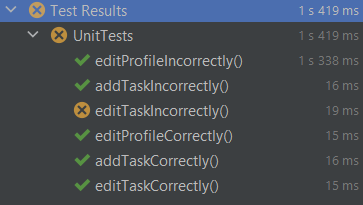
\includegraphics[width=\textwidth]{slike/unitTestRezultati.png}
			\caption{Rezultati ispitivanja komponenti}
		\end{figure}
		
		
		
		
		
		
		
		
		
		
		\subsection{Ispitivanje sustava}
		
		Sustav smo ispitivali pomoću Selenium WebDriver okvira. Selenium WebDriver omogućuje ispitivanje sustava za koji je potrebna interakcija s internetskim preglednikom. Koristili smo Google Chrome preglednik. Ispitali smo funkcionalnosti uređivanja profila, uređivanja zadatka i dodavanja zadatka. Koriste se pomoćna metoda void login(WebDriver driver, String username, String password) za prijavu željenog korisnika u sustav i void logout(WebDriver driver) za odjavu korisnika. U main metodi definirane su potrebne vrijednosti za poziv svake funkcije.
		
		\textbf{Ažuriranje profila}
		
		Cilj prvog testa uspješno je ažuriranje korisnika. Funkcija editProfileCorrectly prvo prijavljuje željenog korisnika (korisničkog imena mhren), pritiskom na gumb otvara profil, odabire opciju za uređivanje, mijenja broj mobitela i mail te sprema promijenjene podatke. Test je uspješan ukoliko su broj mobitela i mail korisničkog profila postali jednaki željenima.
		\begin{verbatim}
			
			public static String editProfileCorrectly(WebDriver driver,String username,
			String password,String newPhone,String newMail) {
				
				  login(driver,username,password);
				
				  driver.findElement(By.id("openProfile")).click();
				  driver.findElement(By.id("editProfile")).click();
				
				  WebElement element = driver.findElement(By.id("brMob"));
				  element.clear();
				  element.sendKeys(newPhone);
				
				  element = driver.findElement(By.id("eMail"));
				  element.clear();
				  element.sendKeys(newMail);
				
				  driver.findElement(By.id("spremi")).click();
				  boolean success=driver.findElement(By.id("mail")).getText().equals(newMail)&&
				  driver.findElement(By.id("mob")).getText().equals(newPhone);
				
				  return "editProfileCorrectly success: " + success;
			}
			
		\end{verbatim}
		Cilj drugog testa neuspješno je ažuriranje korisnika. Na početku funkcije editProfileIncorrectly već smo prijavljeni u sustav. Ponovno otvaramo profil i želimo ga urediti, ovaj 
		put pokušavamo postaviti prazno korisničko ime, što se ne bi smjelo prihvatiti. Uspjehom smatramo ako u određenom vremenu iskoči prozor s upozorenjem koji označava da se podatci nisu promijenili. Ako se prozor pojavi na njemu pritišćemo "U redu". Odjavljujemo trenutnog korisnika zato što nam za idući test treba drugi korisnik.
		\begin{verbatim}
			
			public static String editProfileInorrectly(WebDriver driver){
				  
				  driver.findElement(By.id("editProfile")).click();
				  WebElement element = driver.findElement(By.id("korIme"));
				  element.clear();
				  element.sendKeys(null);
				  driver.findElement(By.id("spremi")).click();
				
				  boolean success;
				
				  try {
					    WebDriverWait wait = new WebDriverWait(driver, 2);
					    wait.until(ExpectedConditions.alertIsPresent());
					    driver.switchTo().alert().accept();
					    success = true;
				  }catch(TimeoutException ex){
					    success = false;
				  }
				
				  driver.findElement(By.id("zatvori")).click();
				  logout(driver);
				  return "editProfileIncorrectly success: " + success;
			}
			
		\end{verbatim}
		\textbf{Dodavanje zadatka}
		
		Želimo uspješno dodati zadatak. U fuknciji addTaskCorrectly prvo se prijavljujemo s korisničkim podatcima koordinatora, pritišćemo gumb za dodavanje zadatka, dajemo mu ime, opis, prioritet i rok te ga spremamo. Uspješni smo ukoliko je broj zadataka na kanban ploči za jedan viši od broja zadataka na ploči prije pokušaja dodavanja zadatka.
		\begin{verbatim}
			
			public static String addTaskCorrectly(WebDriver driver,String username, 
			String password,String taskName,String description,
			TaskPriority priority,String deadline){
				
				  login(driver,username,password);
				
				  int numberOfTasks = driver.findElements(By.id("task")).size();
				  driver.findElement(By.id("addTask")).click();
				
				  driver.findElement(By.id("taskName")).sendKeys(taskName);
				  driver.findElement(By.id("description")).sendKeys(description);
				  driver.findElement(By.id("priority")).sendKeys(priority.toString());
				  driver.findElement(By.id("deadline")).sendKeys(deadline);
				  driver.findElement(By.id("add")).click();
				
				  boolean success=driver.findElements(By.id("task")).size()==numberOfTasks+1;
				  return "addTaskCorrectly success: " + success;
			}
			
		\end{verbatim}
		Želimo neuspješno dodati zadatak. U funkciji addTaskIncorrectly pritišćemo gumb za dodavanje zadatka, upisujemo naziv, opis te prioritet i rok neispravnih oblika. Spremamo podatke. Uspjehom smatramo ako u određenom vremenu iskoči prozor upozorenja koji označuje da zadatak nije dodan. Ako se prozor pojavi na njemu pritišćemo "U redu".
		
		\begin{verbatim}
			
			public static String addTaskIncorrectly(WebDriver driver,String taskName,
			String description){
				
				  driver.findElement(By.id("addTask")).click();
				
				  driver.findElement(By.id("taskName")).sendKeys(taskName);
				  driver.findElement(By.id("description")).sendKeys(description);
				  driver.findElement(By.id("priority")).sendKeys("unknown");
				  driver.findElement(By.id("deadline")).sendKeys("unknown");
				  driver.findElement(By.id("add")).click();
				
				  boolean success;
				
				  try {
					    WebDriverWait wait = new WebDriverWait(driver, 2);
					    wait.until(ExpectedConditions.alertIsPresent());
					    driver.switchTo().alert().accept();
					    success = true;
				  }catch(TimeoutException ex){
					    success = false;
				  }
				  return "addTaskIncorrectly success: " + success;
			}
			
		\end{verbatim}
		\textbf{Ažuriranje zadatka}
		
		Cilj ovog testa uspješno je uređivanje zadatka. Prije poziva funkcije editTaskCorrectly nalazimo se na kanban ploči iz prethodnog testa. Pronalazimo jedan gumb za uređivanje zadatka koji možemo pritisnuti (tj. jedan zadatak koji smo ranije preuzeli te ga imamo pravo urediti). Pritišćemo pronađeni gumb, zadatku mijenjamo opis i spremamo promjene. Uspjehom smatramo ako se nakon određenog vremena nije pojavio skočni prozor s upozorenjem koji bi signalizirao da zadatak nije uspješno promijenjen.
		\begin{verbatim}
			
			public static String editTaskCorrectly(WebDriver driver, String description){
				  
				  ArrayList<WebElement> editButtons=(ArrayList<WebElement>)driver.findElements(
				  By.id("editTask"));
				  for(WebElement editButton:editButtons){
					    if(editButton.isEnabled()){
						      editButton.click();
						      break;
					    }
				  }
				
				  WebElement element = driver.findElement(By.id("description"));
				  element.clear();
				  element.sendKeys(description);
				
				  driver.findElement(By.id("saveTask")).click();
				
				  boolean success;
				  try {
					    WebDriverWait wait = new WebDriverWait(driver, 2);
					    wait.until(ExpectedConditions.alertIsPresent());
					    driver.switchTo().alert().accept();
					    success = false;
				  }catch(TimeoutException ex){
					    success = true;
				  }
				  return "editTaskCorrectly success: " + success;
			}
			
		\end{verbatim}
		Posljednjim testom želimo neuspješno ažurirati zadatak. U funkciji editTaskIncorrectly pritišćemo gumb za uređivanje zadatka, postavljamo prazni prioritet i spremamo promjene. Uspjehom smatramo ako se nakon nekog vremena pojavi skočni prozor koji označava da je nešto pošlo po krivu.
		
		\begin{verbatim}
			
			public static String editTaskIncorrectly(WebDriver driver){
				  
				  ArrayList<WebElement> editButtons=
				  (ArrayList<WebElement>)driver.findElements(By.id("editTask"));
				  for(WebElement editButton:editButtons){
					    if(editButton.isEnabled()){
						      editButton.click();
						      break;
					    }
				  }
				
				  WebElement element = driver.findElement(By.id("priority"));
				  element.clear();
				
				  driver.findElement(By.id("saveTask")).click();
				
				  boolean success;
				  try {
					    WebDriverWait wait = new WebDriverWait(driver, 2);
					    wait.until(ExpectedConditions.alertIsPresent());
					    driver.switchTo().alert().accept();
					  success = true;
				  }catch(TimeoutException ex){
					    success = false;
				  }
				  return "editTaskInorrectly success: " + success;
			}
			
			
		\end{verbatim}
		
		\begin{figure}[H] 
			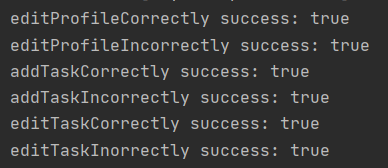
\includegraphics[width=\textwidth]{slike/systemTestRezultati.png}
			\caption{Rezultati ispitivanja sustava}
		\end{figure}
			
			\eject 
		
		
		\section{Dijagram razmještaja}
			
			Dijagrami razmještaja prikazuju topologiju sustava i odnos sklopovskih i programskih dijelova. Olakšavaju nam vizualizaciju razmještaja fizičkog dijela sustava i sklopovlja. Sustav se sastoji od korisničkog i poslužiteljskog računala. Korisnik na svojem računalu preko web preglednika pristupa aplikaciji. Korisničko računalo komunicira s poslužiteljskim računalom preko HTTP veze. Na poslužiteljskom se računalu nalaze HTTP poslužitelj, REST poslužitelj i poslužitelj baze podataka. 
			
			\begin{figure}[H]
				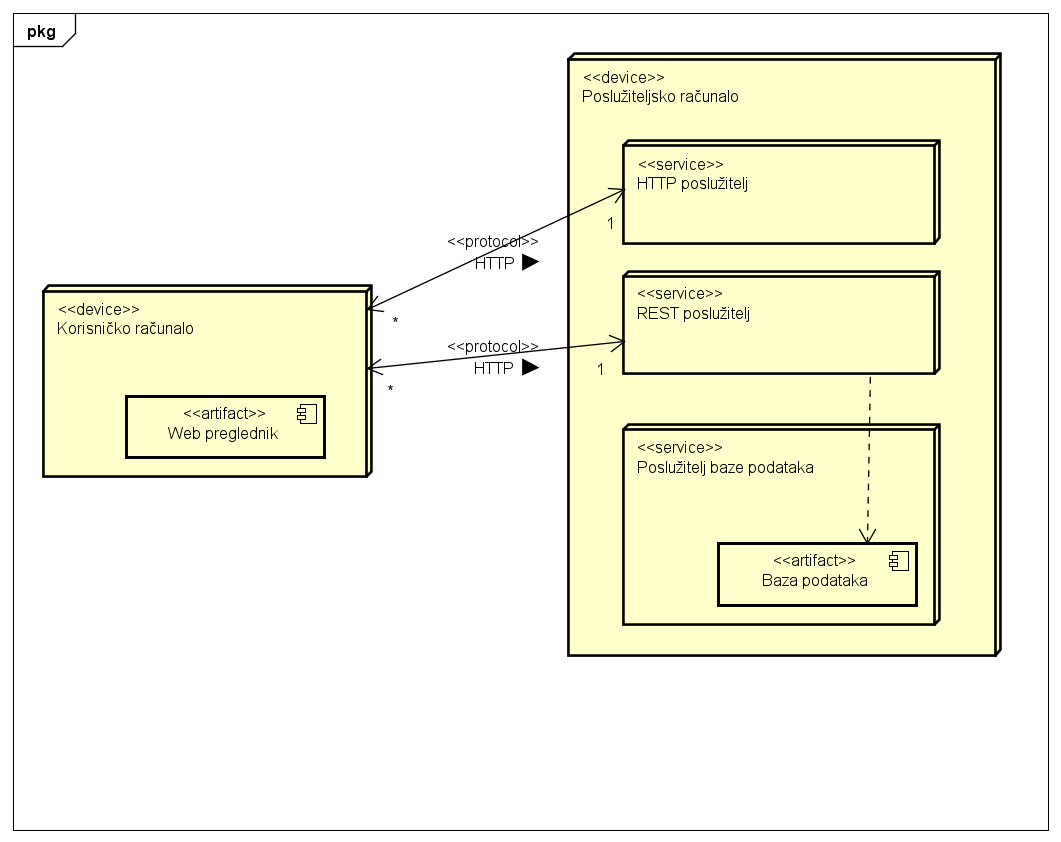
\includegraphics[width=\textwidth]{slike/dijagram_razmjestaja.png}
				\centering
				\caption{Dijagram razmještaja}
				\label{fig:dijagram_razmjestaja}
			\end{figure}
			
			\eject 
		
		\section{Upute za puštanje u pogon}
		
		\subsection{Operacijski sustav}
		Pretpostavlja se operacijski sustav iz Linux obitelji, na primjer \underline{Ubuntu 20.04}\footnote{\url{https://ubuntu.com/}}.
		
		\subsection{Preuzimanje programskog rješenja}
		Potrebno je instalirati paket \texttt{git} naredbom \textbf{sudo apt install git}. Zatim je potrebno pokrenuti naredbu \textbf{git clone \url{https://gitlab.com/henri_ohm/worldpiis.git}} kako bi se preuzelo programsko rješenje. Ovom naredbom će se stvoriti direktorij \texttt{worldpiis} (dalje \$PROJECT\_ROOT) koji sadrži sve potrebne datoteke za pokretanje aplikacije.
		
		\subsection{Baza podataka}
		Potrebnu je preuzeti i instalirati najnoviju verziju paketa PostgreSQL. Pokretanjem naredbe \textbf{sudo apt install postgresql-12} potreban paket se preuzima i instalira, te se stvaraju daemon servisi koji pokreću bazu podataka prilikom pokretanja računala.
		
		\subsection{Konfiguracija poslužitelja baze podataka}
		Ovako instalirana baza podataka sluša zahtjeve sa adrese 127.0.0.1 na vratima 5432. Ovakva konfiguracija dovoljna je za potrebe ovog projekta. Također je potrebno osigurati da u bazi postoji \textbf{korisnik `postgres`} sa \textbf{lozinkom `postgres`}. Potrebno je osigurati i da na računalu postoji korisnik `postgres`, no to bi sama instalacija paketa već trebala osigurati.
		
		\subsection{Konfiguracija baze podataka}
		Sve potrebne tablice, ograničenja i veze će inicijalizirati REST poslužitelj kad se pokrene, pa je potrebno osigurati samo prije navedene uvjete kako bi baza radila.
		
		\subsection{Punjenje baze podataka}
		Za punjenje baze podataka dostupna je skripta na lokaciji \textbf{\$PROJECT\_ROOT/db/fill.sql}. Ova skripta može se pokrenuti tako da se prvo pokrene sučelje s bazom, naredbom \textbf{sudo -i -u postgres psql}, a zatim se pokrene naredba \textbf{\textbackslash i db/fill.sql}. Ovdje se pretpostavlja da je korisnik postavljen u korijenskom direktoriju projekta.
		
		\subsection{Pokretanje baze podataka}
		Baza podataka pokreće se kada se računalo upali, no ukoliko postoje problemi, može se pokrenuti naredba \textbf{sudo systemctl enable postgresql}, koja će omogućiti pokretanje baze prilikom pokretanja računala, te naredba \textbf{sudo systemctl start postgresql} koja će pokrenuti bazu podataka jednom. Prva naredba osigurava pokretanje baze prilikom pokretanja računala.
		
		\subsection{Javna vrata servera}
		Potrebno je osigurati da su vrata 80 i vrata 8080 otvorena javnosti, što je moguće naredbom \textbf{sudo ufw allow 80} i \textbf{sudo ufw allow 8080}. Ovaj postupak omogućuje poslužitelju primanje zahtjeva na ta dva vrata. Vrata 80 su dobro poznata vrata za posluživanje HTTP zahtjeva, a na vrata 8080 dolaziti će zahtjevi na REST poslužitelj.
		
		\subsection{Pokretanje web poslužitelja}
		Prije svega, potrebno je osigurati prisutnost Python interpretatora, što je moguće naredbom \textbf{sudo apt install python3}. Nadalje, da bi se web poslužitelj pokrenuo, potrebno je pozicionirati se u direktorij \textbf{\$PROJECT\_ROOT/web} i pokrenuti naredbu \textbf{sudo python3 -m http.server 80}. Prije toga, potrebno je osigurati da su vrata 80 slobodna, odnosno da nijedan drugi proces ne sluša na tim vratima.
		
		\subsection{Konfiguracija veze s bazom podataka}
		U datoteci \textbf{\$PROJECT\_ROOT/src/main/resources/application.properties} postavljene su iduće konfiguracijske varijable:
		\begin{itemize}
			\item \texttt{spring.datasource.url = jdbc:postgresql://localhost:5432/postgres}
			\item \texttt{spring.datasource.username = postgres}
			\item \texttt{spring.datasource.password = postgres}
		\end{itemize}
		Prva varijabla govori poslužitelju na koji URI treba slati zahtjeve bazi podataka. Druga i treća varijabla govore s kojim korisničkim imenom i lozinkom se ti zahtjevi trebaju slati.
		
		\subsection{Pokretanje REST poslužitelja}
		Prije nego što se pokrene REST poslužitelj, potrebno je osigurati prisutnost Jave 13 i programskog paketa Apache Maven. U tu svrhu, potrebno je pokrenuti naredbu \textbf{sudo apt install openjdk-13 maven}, koja će instalirati oba paketa u jednom potezu. Nakon toga, potrebno je pozicionirati se u korijenski direktorij i pokrenuti naredbu \textbf{mvn -N io.takari:maven:wrapper}, koja će instalirati potreban paket za pokretanje Spring aplikacije. Konačno, u korijenskom direktoriju potrebno je pokrenuti poslužitelj naredbom \textbf{./mvnw spring-boot:run}. Ukoliko su potrebne debugging poruke, moguće je staviti zastavice \underline{-e -X}.  
		
		\subsection{Konfiguriranje adrese spajanja}
		Na početku datoteke \textbf{\$PROJECT\_ROOT/web/app.js} dostupna je varijabla \textbf{REST\_base} koja govori na koju adresu i vrata frontend treba slati zahtjeve da bi dobio REST odgovore. Ova varijabla po potrebi se može mijenjati za lokalno testiranje ili kada se mijenja domena ili adresa aplikacije. 
		
		\subsection{Domena aplikacije}
		Kako bi aplikaciji bilo lakše pristupati, potrebno je registrirati domenu na bilokojem pružatelju domenskih imena. Za potrebe ovog projekta, korišten je \textbf{DuckDNS}\footnote{\url{https://www.duckdns.org/}}.
		
		\subsection{Korištenje aplikacije}
		Nakon svih ovih koraka, aplikacija je upogonjena i dostupna na registriranoj domeni. Aplikacija ovog projekta dostupna je na domeni \textbf{\url{worldpiis.duckdns.org}}.
		\eject 
	\chapter{Zaključak i budući rad}
	Naš zadatak bio je izraditi agilnu platformu s kanban pločom koju bi neka zamišljena tvrtka koristila.
	
	Ideja kanban ploče za upravljanje projektima je sveprisutna u poslovnom svijetu, a dostupna je u alatima poput \underline{Trello}\footnote{\url{https://trello.com/}} i \underline{Asana}\footnote{https://asana.com/}.
	
	Projekt smo proveli u tri faze:
	\begin{enumerate}
		\item početna razrada funkcionalnih i nefunkcionalnih zahtjeva
		\item implementacija zahtjeva i daljnje razrađivanje
		\item testiranje i završno dokumentiranje
	\end{enumerate} 

	Na početku prve faze upoznavali smo ideju aplikacije, razrađivali smo funkcionalne zahtjeve i dogovarali se što sve aplikacija može i treba raditi. U retrospekciji, ova faza provedena je kaotično jer članovi tima još nisu bili svjesni težine projekta i količine posla, a da se provela kvalitetnije implementacija bi bila konceptualno lakša. U prvoj fazi smo se također počeli upoznavati s tehnologijama koje smo koristili. Ni jedan od članova tima nije bio u potpunosti upoznat s tim tehnologijama. Naučili smo da u stvarnosti, prije izrade samog projekta, potrebno je naučiti kako učiti alate, a zatim i naučiti sam alat.
	
	U drugoj fazi projekta krenuli smo sa implementacijom, što je na početku teklo jako sporo jer još nismo bili upoznati s alatima, no kako je vrijeme prolazilo tako smo postajali bolji i implementirali smo zahtjeve sve brže. Također, u ovoj fazi uvidjeli smo propuste u definicijama funkcionalnih i nefunkcionalnih zahtjeva, pa smo naučili biti precizniji u svojim definicijama i uzimati više slučajeva u obzir. 
	
	U trećoj, odnosno posljednjoj fazi, nakon implementacije programskog rješenja, dovršili smo dokumentaciju projekta. Ovaj korak nam je dodatno pomogao u shvaćanju obujma našeg projekta, i ukazao nam na arhitekturalne probleme koje nismo predvidjeli. Također, testiranjem smo ustanovili da sustav ima par grešaka, a najveća od tih je da REST API vraća prvi ugnježđeni objekt u potpunosti, a sve ostale vraća samo preko njihovih identifikatora.
	
	Članovi tima su prije projekta bili upoznati s Javom i NodeJS-om, pa bi odabirom tih tehnologija umjesto AngularJS-a pomogao pri ubrzanju razvoja aplikacije. 
	
	Naučili smo važnost koordinacije i komunikacije među članovima tima. Nekad članovi nisu bili dobro koordinirani pa bi jedni implementirali funkcionalnost na ovaj, a drugi na onaj način. Naučili smo meke vještine povezane s projektima općenito, kao što je korištenje alata \texttt{git}, pisanje značajnih commit poruka, korištenje GitLab-a, te poštivanje unaprijed definiranih obrazaca programiranja. 
	
	Najviše od svega, naučili smo značenje vremenske koordiniranosti u grupnom radu. Projekti poput ovoga vremenski su zahtjevni i ponekad se može dogoditi da jedan modul programskog rješenja kasni za drugim, pa drugi ne može nastaviti svoj razvoj. U ovakvim slučajevima, iznimno je važno vremenski se uskladiti unutar tima kako bi se takve neučinkovitosti izbjegle. 
	
	Od definiranih funkcionalnih zahtjeva, uspjeli smo implementirati korisnički login, dodavanje i mijenjanje zadataka, preuzimanje zadataka, pregled kanban ploča timova od strane uprave i koordinatora, integraciju GoogleCalendar-a za sastanke i izmjenu profila zaposlenika.
	
	Prije spomenuti bug primijetili smo tek na kraju izrade projekta i nismo imali dovoljno vremena kako bi ga popravili. Bug smo primijetili tako kasno jer smo do tada rukovali sa lijepim podacima i nismo imali priliku uvidjeti pogrešku. Iz ovoga smo naučili da temeljito testiranje sustava treba provoditi od samog početka, koliko je to god moguće. 
	
	U budućnosti bismo mogli popraviti taj bug, zatim mogli bismo omogućiti upravljanje sjednicom, ćime bismo postigli mogućnost da više korisnika istovremeno koristi našu aplikaciju bez problema, i u više sjednica odjednom. Također, mogli bismo prolijepšati korisničko sučelje, implementirati više statusa zadataka, proširiti profil korisnika da sadrži druge korisničke podatke, omogućiti upravi pregled profila i aktivnosti pojedinih zaposlenika, i slično.

	Zaključno, zahvaljujući iskustvima i znanjima koja smo stekli na ovom projektu, kad bismo krenuli iz početka, napravili bismo mnogo bolji projekt mnogo brže.
	\eject 

	\chapter*{Popis literature}
		\addcontentsline{toc}{chapter}{Popis literature}
		
		
		\begin{enumerate}
			
			
			\item  Programsko inženjerstvo, FER ZEMRIS, \url{http://www.fer.hr/predmet/proinz}
			
			\item  I. Sommerville, "Software engineering", 8th ed, Addison Wesley, 2007.
			
			\item  T.C.Lethbridge, R.Langaniere, "Object-Oriented Software Engineering", 2nd ed. McGraw-Hill, 2005.
			
			\item  I. Marsic, Software engineering book``, Department of Electrical and Computer Engineering, Rutgers University, \url{http://www.ece.rutgers.edu/~marsic/books/SE}
			
			\item  The Unified Modeling Language, \url{https://www.uml-diagrams.org/}
			
			\item  Astah Community, \url{http://astah.net/editions/uml-new}
			
			\item  Java Spring dokumentacija, \url{https://spring.io/projects/spring-framework}
			
			\item  AngularJS dokumentacija, \url{https://docs.angularjs.org/api}
		\end{enumerate}
		
		 
	
	
	\begingroup
	\renewcommand*\listfigurename{Indeks slika i dijagrama}
	%\renewcommand*\listtablename{Indeks tablica}
	%\let\clearpage\relax
	\listoffigures
	%\vspace{10mm}
	%\listoftables
	\endgroup
	\addcontentsline{toc}{chapter}{Indeks slika i dijagrama}


	
	\eject 
		
	\chapter*{Dodatak: Prikaz aktivnosti grupe}
		\addcontentsline{toc}{chapter}{Dodatak: Prikaz aktivnosti grupe}
		
		\section*{Dnevnik sastajanja}
		\def\djo{Đokić}
		\def\fuc{Fučec}
		\def\hab{Habuš}
		\def\hre{Hren}
		\def\juk{Jukić}
		\def\luk{Lukenda}
		\def\pav{Pavlic}
		\begin{packed_enum}
			\item  sastanak
			
			\item[] \begin{packed_item}
				\item Datum: 5. listopada 2020.
				\item Prisustvovali: \djo, \fuc, \hre, \hab, \juk, \luk, \pav
				\item Teme sastanka:
				\begin{packed_item}
					\item  sastanak s asistentom
					\item  analiza zadatka
					\item  osnovne dileme funkcionalnosti
				\end{packed_item}
			\end{packed_item}
			
			\item  sastanak
			\item[] \begin{packed_item}
				\item Datum: 12. listopada 2020.
				\item Prisustvovali: \djo, \hab, \hre, \juk, \pav
				\item Teme sastanka:
				\begin{packed_item}
					\item  sastanak s asistentom
					\item  odabir alata i tehnologija
				\end{packed_item}
			\end{packed_item}
		
			\item  sastanak
			\item[] \begin{packed_item}
				\item Datum: 14. listopada 2020.
				\item Prisustvovali: \djo, \fuc, \hab, \hre, \juk, \luk, \pav
				\item Teme sastanka:
				\begin{packed_item}
					\item  temeljitiji opis aplikacije
					\item  definiranje funkcionalnih zahtjeva i aktora
					\item  definiranje ostalih zahtjeva
				\end{packed_item}
			\end{packed_item}
		
			\item  sastanak
			\item[] \begin{packed_item}
				\item Datum: 19. listopada 2020.
				\item Prisustvovali: \fuc, \hab, \hre, \juk, \pav
				\item Teme sastanka:
				\begin{packed_item}
					\item  raspodjela poslova za razvoj aplikacije
					\item  idejna razrada arhitekture aplikacije
				\end{packed_item}
			\end{packed_item}
		
			\item  sastanak
			\item[] \begin{packed_item}
				\item Datum: 26. listopada 2020.
				\item Prisustvovali: \djo, \fuc, \hab, \hre, \juk
				\item Teme sastanka:
				\begin{packed_item}
					\item  razrada baze s asistentom
					\item  razrada arhitekture backenda
					\item  definicija izgleda stranica
				\end{packed_item}
			\end{packed_item}
			
			\item  sastanak
			\item[] \begin{packed_item}
				\item Datum: 2. studenog 2020.
				\item Prisustvovali: \fuc, \hab, \hre, \juk, \pav
				\item Teme sastanka:
				\begin{packed_item}
					\item  REST kontroleri
					\item  dublja razrada frontenda
					\item  rasprava o idejama za v2.0
				\end{packed_item}
			\end{packed_item}
		
			\item  sastanak
			\item[] \begin{packed_item}
				\item Datum: 9. studenog 2020.
				\item Prisustvovali: \djo, \fuc, \hab, \hre, \juk, \luk, \pav
				\item Teme sastanka:
				\begin{packed_item}
					\item  demonstracija aplikacije asistentu
					\item  dogovor i raspored zadataka za poliranje verzije 1.0 aplikacije
					\item  razumijevanje frontenda
				\end{packed_item}
			\end{packed_item}
		
			\item sastanak
			\item[] \begin{packed_item}
				\item Datum 7. prosinca 2020.
				\item Prisustvovali: \djo, \fuc, \hre, \juk, \pav
				\item Teme sastanka:
				\begin{packed_item}
					\item  raspodjela poslova
				\end{packed_item} 
			\end{packed_item}
		
			\item sastanak
			\item[] \begin{packed_item}
				\item Datum 30. prosinca 2020.
				\item Prisustvovali: \djo, \hab, \hre, \juk
				\item Teme sastanka:
				\begin{packed_item}
					\item  raspodjela poslova do $\alpha$-inačice
				\end{packed_item} 
			\end{packed_item}
		
			\item sastanak
			\item[] \begin{packed_item}
				\item Datum 8. siječnja 2021.
				\item Prisustvovali: \djo, \fuc, \hab, \hre, \juk, \luk, \pav
				\item Teme sastanka:
				\begin{packed_item}
					\item  demonstracija $\alpha$-inačice
					\item  raspodjela poslova do završetka projekta
				\end{packed_item} 
			\end{packed_item}
			%
			
		\end{packed_enum}
		
		\eject
		\section*{Tablica aktivnosti}
						
			
			\begin{longtabu} to \textwidth {|X[7, l]|X[1, c]|X[1, c]|X[1, c]|X[1, c]|X[1, c]|X[1, c]|X[1, c]|}
								
				\cline{2-8} \multicolumn{1}{c|}{\textbf{}} &     \multicolumn{1}{c|}{\rotatebox{90}{\textbf{Miho Hren }}} & \multicolumn{1}{c|}{\rotatebox{90}{\textbf{Nikola Đokić }}} &	\multicolumn{1}{c|}{\rotatebox{90}{\textbf{Borna Fučec }}} &	\multicolumn{1}{c|}{\rotatebox{90}{\textbf{Luka Habuš }}} &
				\multicolumn{1}{c|}{\rotatebox{90}{\textbf{Ana-Petra Jukić }}} &
				\multicolumn{1}{c|}{\rotatebox{90}{\textbf{Ana Lukenda }}} &	\multicolumn{1}{c|}{\rotatebox{90}{\textbf{Evelyn Pavlic }}} \\ \hline 
				\endfirsthead
				
				
				\cline{2-8} \multicolumn{1}{c|}{\textbf{}} &     \multicolumn{1}{c|}{\rotatebox{90}{\textbf{\hre }}} & \multicolumn{1}{c|}{\rotatebox{90}{\textbf{\djo }}} &	\multicolumn{1}{c|}{\rotatebox{90}{\textbf{\fuc }}} &	\multicolumn{1}{c|}{\rotatebox{90}{\textbf{\hab }}} &
				\multicolumn{1}{c|}{\rotatebox{90}{\textbf{\juk }}} &
				\multicolumn{1}{c|}{\rotatebox{90}{\textbf{\luk }}} &	\multicolumn{1}{c|}{\rotatebox{90}{\textbf{\pav }}} \\ \hline
				\endhead
				
				
				\endfoot
							
				 
				\endlastfoot
				
				Upravljanje projektom 		&  6&  &  &  &  &  & \\ \hline

				Opis projektnog zadatka 	&  &  &  &  &  &  & 4 \\ \hline
				
				Funkcionalni zahtjevi       &  &  &2  &  &2  &  &  \\ \hline
				Opis pojedinih obrazaca 	&  &  &  &  &  & 2 &  \\ \hline
				Dijagram obrazaca 			&  &  &  &  &  & 2 &  \\ \hline

				Sekvencijski dijagrami 		&  & 4 &  &  &  &  &  \\ \hline
				Opis ostalih zahtjeva 		&  1&  &  &  &  &  &  \\ \hline

				Arhitektura i dizajn sustava	 &  3&  &  &  &  &  &  \\ \hline
				Baza podataka				&  5&  &  &  &  &  &   \\ \hline
				Dijagram razreda 			&  2&  &  &  &  &  &   \\ \hline
				Dijagram stanja				&  & 3 &  &  &  &  &  \\ \hline

				Dijagram aktivnosti 		&  &  &  &  2&  &  &  \\ \hline
				Dijagram komponenti			&  &  &  &  2&  &  &  \\ \hline
				Korištene tehnologije i alati 		&  &  &  &  1&  &  &  \\ \hline
				Ispitivanje programskog rješenja 	&  &  &  &  &  & 6 &  \\ \hline
				Dijagram razmještaja			&  &  &2  &  &  &  &  \\ \hline
				Upute za puštanje u pogon 		&  2&  &  &  &  &  &  \\ \hline 
				Dnevnik sastajanja 			&  1&  &  &  &  &  &  \\ \hline
				Zaključak i budući rad 		&  &  &  &  1&  &  &  \\  \hline
				Popis literature 			&  &  &  &  &  &  &  \\  \hline
				&  &  &  &  &  &  &  \\ \hline \hline

				\textit{Izrada početne stranice} 				&  & 4 & 4 &  2& 25 & 2 &  25\\ \hline 
				\textit{Izrada baze podataka} 		 			& 5 &  &  &  &  &  & \\ \hline 
				\textit{Spajanje s bazom podataka} 							&  4& 4 & 4 &  &  & 2 &  \\ \hline
				\textit{Back end} 							& 15 &  & 3 &  &  &  & 2 \\  \hline

				 							&  &  &  &  &  &  &\\  \hline
				
				
			\end{longtabu}
					
					
		\eject
		\section*{Dijagrami pregleda promjena}
		
		\begin{figure}[H]
			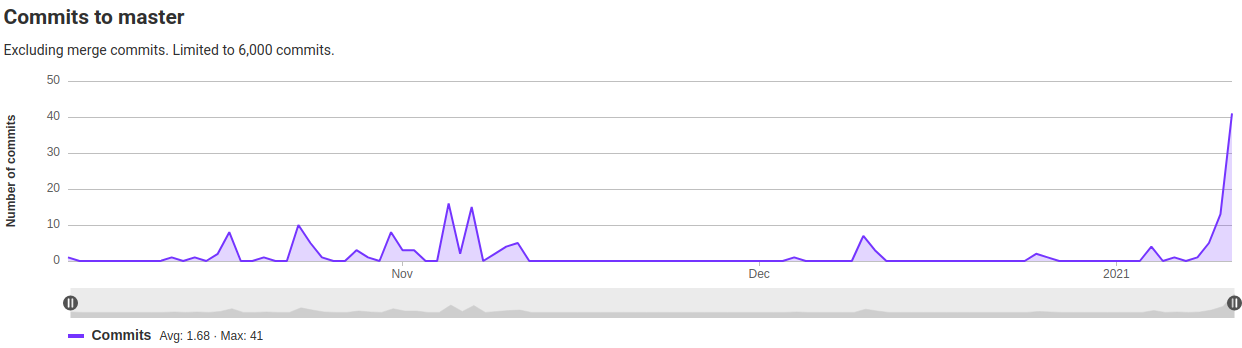
\includegraphics[scale=0.3]{slike/master.png}
			\centering
			\caption{Promjene na master grani}
			\label{fig:master}
		\end{figure}
	
		\begin{figure}[H]
			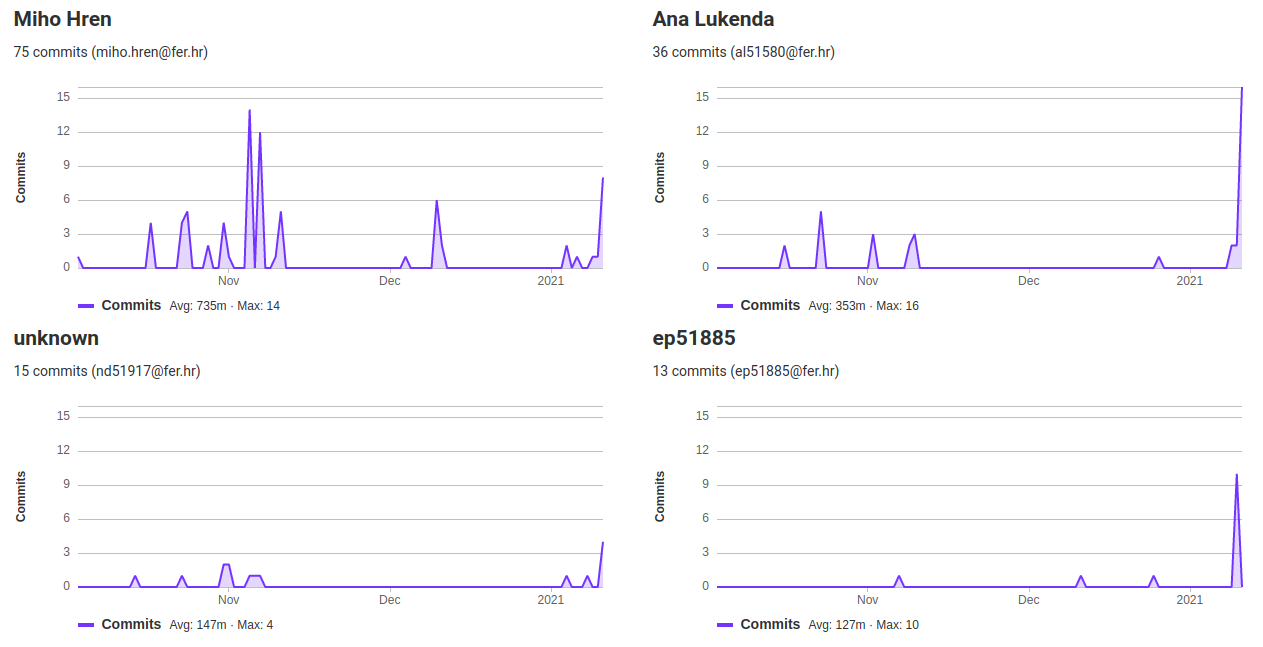
\includegraphics[scale=0.3]{slike/promjene1.png}
			\centering
			\caption{Aktivnosti članova tima}
			\label{fig:promjene1}
		\end{figure}

		\begin{figure}[H]
			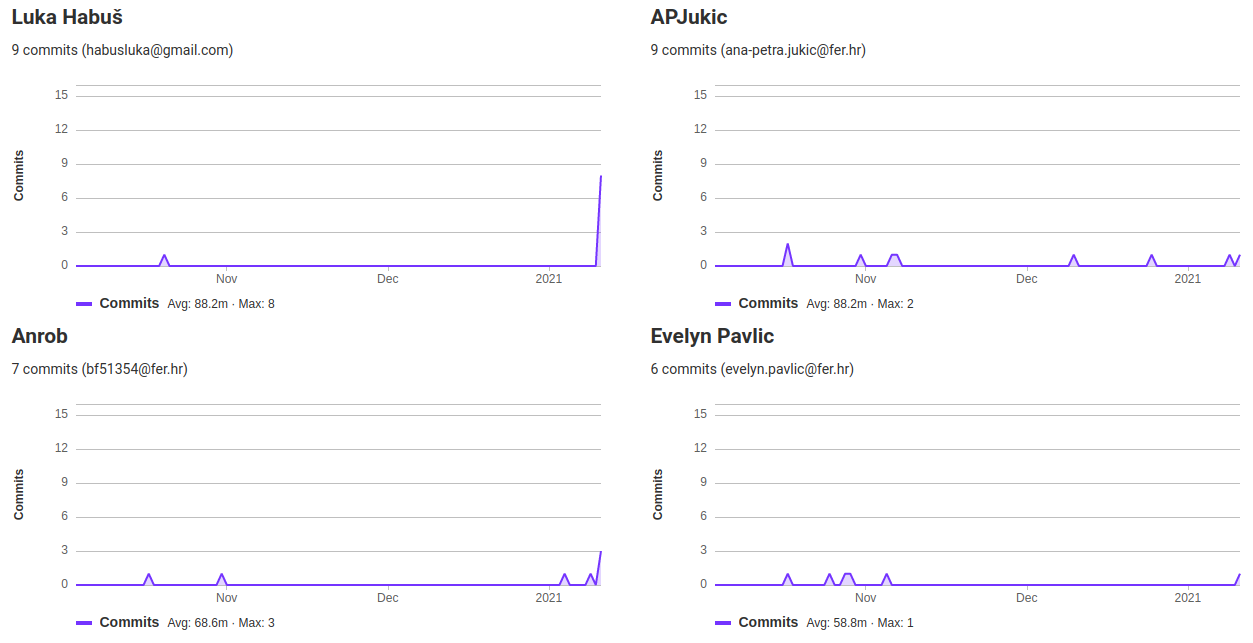
\includegraphics[scale=0.3]{slike/promjene2.png}
			\centering
			\caption{Aktivnosti članova tima}
			\label{fig:promjene2}
		\end{figure}


\end{document} %naredbe i tekst nakon ove naredbe ne ulaze u izgrađen dokument 


